\documentclass[12pt,letterpaper ,oneside , openright]{book}
\usepackage{thesis}
%para desarrollo
	%\usepackage{showframe}
	%\includeonly{usingTheLibrary_chapter,usingthelibrary/compresibilityFactor,usingthelibrary/fugacity,usingthelibrary/volume,apendixEquations,usingthelibrary/parameters}     
	%\includeonly{usingTheLibrary_chapter}
%--              
\begin{document}      
	\begin{titlepage}
	\begin{minipage}[c][9in][s]{1in}
	\centering
	
\includegraphics[width=1in]{Escudo-UNAM}\\[10pt]
	\hskip 2pt\vrule width 2pt height 6.7in
	\hskip 1mm\vrule width 1pt height 6.7in\\[10pt]
	
\includegraphics[width=1in]{images/FQ.jpg}
	\end{minipage}\hskip 10pt
	\begin{minipage}[c][\textheight][s]{5.125in}
	\centering
	{\textsc{ \large{Universidad Nacional Autónoma De México}}}
	\vspace{3mm}\hrule height2pt
	\vspace{1mm}\hrule height1pt
	\vspace{3mm}
	\textsc{Facultad De Química}\\[3cm]
	\textsc{\Large Desarrollo de una librería en java para el cálculo de propiedades de sustancias con ecuaciones de estado cúbicas}\\[3cm]
	\makebox[8cm][s]{\Huge T E S I S}\\[8pt]
	\textsc{ que para obtener el título de }\\[3pt]
	\textsc{ Ingeniero Químico}\\[1cm]
	\textsc{ presenta: }\\[0.3cm]
	\textsc{ Hugo Redon Rivera }\\[0.5cm]
	\vfill
	{\scshape {México, D.F.} \hfill{2014} }	
	\end{minipage}
\end{titlepage}
\newpage
\begin{minipage}[c][\textheight][s]{5.125in}
JURADO ASIGNADO:\\[0.5cm]

PRESIDENTE:		Profesor:\\
VOCAL: 		Profesor:\\
SECRETARIO:		Profesor:\\
1er.  SUPLENTE: 	Profesor:\\
2° SUPLENTE:		Profesor:\\[0.5cm]

\begin{center}
	SITIO DONDE SE DESARROLLÓ EL TEMA:\\
	\textsc{Facultad de Química}\\[3cm]


	\rule{6cm}{1pt}\\
	\textsc{asesor del tema: Dr. Enrique Rodolfo Bazúa Rueda.} \\[3cm]


	\rule{6cm}{1pt}\\
	\textsc{SUSTENTANTE:Hugo Redon Rivera.} 
\end{center}
\end{minipage}
%Portada -Hecho
	\tableofcontents	
	\chapter{Objetivos}

\begin{itemize}
	\item Desarrollar una biblioteca escrita en el lenguaje de java para realizar:
	\begin{itemize}
		\item El cálculo de propiedades de sustancias puras y mezclas con ecuaciones de estado cúbicas.
		\item Cálculos de equilibrio Líquido-Vapor.
		\item La estimación de parámetros de expresiones de $\alpha$ para el cálculo de la constante $a$ de la ecuación de estado cúbica.
		\item La estimación de parámetros binarios de las reglas de mezclado para el cálculo de las constantes $a$ y $b$ para mezclas.
	\end{itemize}
	\item La biblioteca a desarrollar deberá ser versátil, robusta, simple de usar y fácilmente expandible.
	\item Desarrollar una interfaz de usuario que exponga las funciones de la librería.
	\item Proponer un medio de difusión de la librería, que sea capaz de involucrar a cualquier persona interesada en modificar y extender la librería.
\end{itemize}

\chapter{Introducción}

	Esta tesis trata sobre el uso de métodos computacionales para el cálculo de propiedades volumétricas y puntos de equilibrio Líquido-Vapor con ecuaciones de estado cúbicas. 

	Como resultado se ha escrito una biblioteca de clases en java denominada \textbf{Materia}.

	El diseño de la biblioteca en conjunto con las herramientas que se describen en la sección \ref{chap:tools} hacen de este trabajo una plataforma para el desarrollo de aplicaciones de simulación y modelado de procesos quimicos industriales.

	El presente trabajo propone un procedimiento para el desarrollo de futuras aplicaciones. Para lo cual se ha dotado de ciertas características a la biblioteca \textbf{Materia} asegurando el funcionamiento del proceso propuesto.

	La biblioteca \textbf{Materia} se ha escrito para que su utilizacióń sea sencilla y no se requieran grandes conocimientos sobre programación. El capítulo \ref{chap:libraryUse} muestra como utilizar la estructura de clases para realizar los cálculos de propiedades y de equilibrio, mostrando pequeños fragmentos de código.

	El capítulo \ref{chap:libraryExtension} muestra como extender la biblioteca de clases, guía en el proceso de creación de nuevas reglas de mezclado, expresiones de $\alpha$, etc. Este capítulo supone un conocimiento mas avanzado en temas de programación orientada a objetos.

	Se ha creado una página de internet para permitir el uso de la librería \textbf{Materia} a través de una interfaz de usuario, el capítulo \ref{chap:webPage} documenta las funciones de la página. También es posible extender las funciones de la página de internet, sin embargo son necesarios conocimientos que estan fuera del alcance de esta tesis. El apéndice \ref{chap:webTools} describe las tecnologías utilizadas para la creación de la página de internet, y una breve descripción de su estructura.
	%\marginpar{Explicación de las ecuaciones y cálculos que se realizan,Versatilidad del programa,Descripción de la estructura de la tesis,Alcance de la aplicación}
	%Objetivos -Hecho
	\chapter{Herramientas}
	\section{Java}
		Un lenguaje simple, orientado a objetos, distribuido, interpretado, robusto, de arquitectura neutral, portátil, de alto rendimiento, seguro, multiproceso y dinámico.\cite{java} 

		Definición dada por James Gosling \footnote{Considerado creador del lenguaje Java}  en la fecha de su primer publicación (1995). 

		\begin{description}
		\item{Simple:} Una de las razones mas importantes por las que se decidió programar la librería en este lenguaje es que java evita al programador la necesidad de realizar tareas de índole técnico sobre la computadora, como por ejemplo el almacenamiento de los datos en la memoria. Esto permite al programador concentrarse en el area de estudio deseada.

		\item{Orientado a objetos:}
		Sin duda la perspectiva orientada a objetos de java es otro gran atractivo para las ciencias e ingenierías. La división y clasificación de las ramas de estudio permiten concentrarnos en todos y cada uno de los aspectos importantes sobre el tema. De igual manera la division de un programa en objetos nos permite concentrarnos en los aspectos y actividades importantes. Tómese como ejemplo la clasificación de la materia en homogénea y heterogénea, el aspecto importante en esta clasificación es la presencia de uno o más estados de agregación en el sistema, se puede pensar así en un cálculo de equilibrio Líquido-Vapor para un sistema heterogéneo, pero no para un sistema homogéneo.

		\item{Distribuido:}
		Java es una de las principales herramientas para el desarrollo web, un invento solo comparable con la imprenta. Su importancia radica en su capacidad de difusión masiva. La creación de un servicio o cualquier producto es tan importante como su difusión. En conjunto con la librería de funciones se ha creado un sitio web donde se exponen algunas de las funciones mas importantes de la librería.

		\item{De arquitectura neutra:}
		Java es multiplataforma, lo cual significa que puede ser ejecutado en la gran mayoría de los sistemas operativos existentes en el mercado actual.

		\end{description}

	\section{JUnit}

		Esta librería de funciones \footnote{Librería de funciones es una traducción de ``java class library'', que es el nombre del tipo de proyecto del presente trabajo. Una mejor definicion sería una ``Estructura de objetos''} ha sido creada con la idea de expandirse y ser escrita por cualquier persona interesada en ello.Es muy importante mantener una evidencia del funcionamiento de la librería. El uso de la tecnología JUnit es una forma para asegurar que los cambios introducidos al programa no han afectado el funcionamiento esperado de la libreria.

		Al momento de escribir este trabajo la librería cuenta con mas de 100 pruebas que definen un funcionamiento.

		\subsection{Desarrollo basado en pruebas}
	\section{Git}

		Git es un sistema de gestión y distribución de código fuente. Permite llevar un registro de los cambios realizados, utilizar las diferentes versiones, y compartir los cambios entre usuarios.

	\section{GitHub}

		GitHub es un servicio de depósitos de repositorios Git. Es un sitio donde se puede guardar el código fuente, es muy fácil contribuir al proyecto y compartir los cambios propuestos, es accesible a todo el público.

	\section{Maven}

		Maven es una herramienta de construcción de código, una de sus grandes ventajas es que puede descargar de manera segura versiones compiladas de proyectos con unas pocas lineas de código. Mas adelante se detallara el proceso de uso.

	\section{Netbeans}
		NetBeans es un entorno de desarrollo integrado para el desarrollo principalmente con Java, pero también con otros lenguajes, en particular, PHP, C / C++, y HTML5. También es una estructura la plataforma de aplicaciones para aplicaciones de escritorio Java y otros.
	

	\section{Openshift}
		OpenShift es una plataforma de programación en la nube orientada a servicios de Red Hat. Una versión para la nube privada se llama OpenShift Enterprise. El software que ejecuta el servicio se encuentra bajo el nombre "OpenShift Origin" de código abierto y está disponible en GitHub.

	\section{Wildfly}
		WildFly, anteriormente conocido como "JavaBeans Open Source Software Application Server" es un servidor de aplicaciones que implementa la plataforma Java, Enterprise Edition. JBoss está escrito en Java y como tal es multiplataforma: utilizable en cualquier sistema operativo que soporte Java

	\section{GNU GENERAL PUBLIC LICENSE Version 2}

		"GNU GENERAL PUBLIC LICENSE" es una licencia libre, sin derechos para software y otro tipo de obras. Pretende garantizar la libertad de compartir y modificar todas las versiones de un programa - para asegurarse de que sigue siendo software libre para todos sus usuarios.
		
	\section{Idioma}

		Existen dos razones por la que se ha elegido el idioma inglés para expresar las funciones de la librería. La primer razon y las mas importante, es que java ha sido escrito en inglés y por lo tanto las estructuras de control y palabras reservadas. Pongamos como ejemplo el siguiente fragmento de código.

\begin{lstlisting}
public boolean isItADog(Pet pet){
	if ( pet.getSpeciesName().equals("Canis lupus familiaris")) {
		return true;
	}else{
		return false;
	}
}
\end{lstlisting}

	El fragmento de código pretende conocer si el nombre de la especie de la mascota es el nombre científico "Canis lupus familiaris", si es asi devuelve verdadero, de lo contrario falso. Veamos ahora la versión en español para el mismo fragmento de código.

\begin{lstlisting}
public boolean esUnPerro(Mascota mascota){
	if ( mascota.getNombreDeLaEspecie().equals("Canis lupus familiaris")){
		return true;
	}else{
		return false;
	}
}
\end{lstlisting}

	En inglés, el order de las palabras denota la diferencia entre una pregunta y una afirmación, de modo que el nombre del método en inglés claramete indica la pregunta "Is it a Dog?" cuando en español la diferencia entre la pregunta y la afirmación debe ser escrita con un signo de interrogación "¿Es un perro?" sin ellos el nombre del metodo puede parecer la afirmación "Es un perro!".

	También puede notarse el nombre del método "getNombreDeLaEspecie", el prefijo "get" es una convención en java que significa recuperar, se usa para obtener el valor de la variable que continúe al prefijo, sin el prefijo estaríamos restringiendo la funcionalidad de la librería.

	Puede apreciarse que la lectura de la línea en ingles es fluida.No existe la necesidad de realizar traducciones. Aunque parezca trivial en este ejemplo, en porciones mas grandes de código la diferencia es bastante notable.

	Quiero hacer notar que en ningún momento se intenta hacer una comparación sobre los idiomas, sino señalar el beneficio de la fluidez que se obtiene al no mezclarlos.

	%Sobre java y herramientas -Hecho
	\chapter{Instalación}

  Para instalar la biblioteca \textbf{Materia} es necesario saber que tipo de trabajo se desea realizar con ella:
  \begin{itemize}
    \item Crear una aplicación que emplea las funciones ya definidas en la biblioteca.
    \item Crear una nueva funcionalidad de la biblioteca.
  \end{itemize}

  Por ejemplo si se desea escribir una aplicación que realize diagramas de presión contra volumen molar usando ecuaciones de estado cúbicas, solo será necesario instalar la forma compilada según la sección \ref{sec:compiledinstall}. Ya que las funciones para calcular la presión y el volumen molar con ecuaciones de estado cúbicas existen en la biblioteca , no será necesario modificar el código fuente, por lo tanto no es necesaria la instalación del código fuente. En cambio si se desea utilizar ecuaciones viriales para realizar los diagramas de presión, se deberán realizar las dos instalaciones descritas en este capítulo, ya que las ecuaciones viriales no forman parte del alance de esta tesis, la librería debera ser extendida para incluir dichas ecuaciones, una vez hecha la extensión al código fuente , la versión compilada puede ser empleada para realizar la aplicación que realice los diagramas.


  \section{Para uso de la librería (compilado)}\label{sec:compiledinstall}

      Existen dos formas de utilizar la librería Materia en una aplicación java:
    Descargar el archivo .jar y agregarlo al folder /lib de la aplicación ó desde maven utilizando el archivo pom.xml.

    La librería existe como un archivo .jar, se puede descargar desde la página creada para su difusión \url{ingenieria-eqpro.rhcloud.com}, o automáticamente desde los servidores de sonatype haciendo uso de maven.

    Si se realiza la instalación manual la ubicación de la librería depende de la estructura del proyecto, por ejemplo para una aplicación web los archivos jar deberán ser agregados en el folder dentro del proyecto src/main/webapp/WEB-INF/lib.

    Utilizando maven solo deberán agregarse las siguientes lineas de código al archivo pom.xml.

    \begin{lstlisting}[language=XML,morekeywords={repositories,
    repository,id,name,url,groupId,artifactId,dependencies,dependency}]
<dependencies>
  <dependency>
   <groupId>com.github.hugoredon</groupId>
   <artifactId>materia</artifactId>
   <version>1</version>
  </dependency>
</dependencies>
\end{lstlisting}

    En el apéndice \ref{sec:manualInstall} se ejemplifica la instalación manual y en el apéndice \ref{sec:mavenInstall} se muestra la instalación vía maven, para una aplicación de escritorio.


  \section{Para extender o modificar la librería (código fuente)}

    El código fuente de la librería se expone de manera pública en la página \url{https://github.com/HugoRedon/Materia}, bajo la licencia GNU GENERAL PUBLIC LICENSE Version 2.
  
    Para poder participar en el proyecto será necesario obtener de manera gratuita una cuenta en github, realizar una copia o clon \footnote{En github a una copia de un proyecto se conoce como ``Fork''} de la librería  a la nueva cuenta, copiar el código fuente a la computadora haciendo uso de git,realizar los cambios y agregarlos a la cuenta en GitHub  \footnote{El procedimiento hace uso de los comandos `git clone', `git commit' y `git push', que son explicados con mas detalle en el apéndice \ref{chapgithub}} ,finalmente hacer una petición para integrar los cambios a la librería original ``Pull request'', y si los cambios son aceptados, se habrá logrado la participación al proyecto. El proceso se detalla en el apéndice \ref{chap:github}.



%Sobre la instalación Hecho
	\chapter{Uso de la librería}\label{chap:libraryUse}
	
	Dada la extensión de la librería, no resulta posible ni deseable mostrar el código fuente completo\footnote{El código completo puede ser consultado y descargado desde la página \url{https://github.com/HugoRedon/Materia}. El apéndice \ref{chap:github} guía al lector en el procedimiento de modificación o extensión del código fuente.}, en este capítulo se presentan pequeños fragmentos de código que muestran la forma de utilizar la librería y su estructura.
		
	La clase `Cubic' realiza cálculos de presión, fugacidad, factor de compresibilidad y adimensionamiento de los parámetros $a$ y $b$, pero no calcula los parámetros $a$ y $b$.Para calcular los parámetos $a$ y $b$ existen las clases `Substance' y `Mixture' que definen el cálculo de los parámetros para un compuesto puro o para una mezcla respectivamente. 

	Las clases `Substance' y `Mixture' tienen en común los métodos `calculate\_a\_cubicParameter', `calculate\_b\_cubicParameter', ademas de otros que se condensan en la clase `Homogeneous'.La clase `Homogeneous' utiliza los cálculos de los parámetros de la ecuación cúbica y la clase cúbic para finalmente realizar el cálculo de la fugacidad, presión ,factor compresibilidad, entalpía, entropía y energía libre de Gibbs.

	La clase `Homogeneous' no realiza cálculos de equlibrio, ya que la clase representa una sola fase. Para realizar cálculos de equilibrio existe la clase `Heterogeneous' que contiene dos fases una líquida y una vapor. A través de los cálculos de fugacidad de cada fase y empleando un algoritmo numérico se pueden realizar los cálculos de equilibrio Líquid-Vapor.


	Las secciones del capítulo:
	\begin{itemize}
		\item{Sección} \ref{sec:units} Se definen las unidades que emplearan durante todo el capítulo.
		\item{Sección} \ref{sec:cubic}  La clase `Cubic' realiza cálculos de presión, fugacidad, factor de compresibilidad y volumen molar.
		\item{Sección} \ref{sec:compounds} La clase `Compound' para definir y utilizar las propiedades del compuesto puro dentro de la librería.
		\item {Sección} \ref{sec:parameters} La clase `Homogeneous' y sus implementaciones `Substance' y `Mixture' para calcular los parámetros de la ecuación cúbica.
		\item {Sección} \ref{sec:homogeneous} La clase `Homogeneous' para realizar cálculos de entalpía, entropía y energía libre de Gibbs.
		\item {Sección} \ref{sec:heterogeneous} La clase `Heterogeneous' y sus implementaciónes `HeterogeneousSubstance' y `HeterogeneousMixutre' para realizar cálculos de equilibrio Líquido-Vapor.
	\end{itemize}
%hecho
 
		\section{Sistema de Unidades}\label{sec:units}

Las unidades que utiliza la librería se muestran en la tabla \ref{tab:units}.
Durante este escrito se utilizarán las mismas unidades, a menos que se indique lo contrario.


\begin{table}[!h]
	\centering
	\caption{Sistema de unidades empleado por la librería}\label{tab:units}
	\begin{tabular}{ |c| c|c|}
		\hline
			Propiedad & Unidad &\\
		\hline
			Presión & $Pa$ & Pascal\\
			Temperatura & $K$ & Kelvin\\
			Volumen molar & $\frac{m^3}{kg}$ & Metro cúbico sobre kilogramo\\

		\hline
	\end{tabular}
\end{table}%hecho
		\section{Ecuación de estado cúbica}\label{sec:cubic}

	La ecuación de estado cúbica representada por la clase `Cubic', permite realizar los cálculos de: 
	\begin{itemize}	\itemsep0ex
		\item Presión
		\item Factor de compresibilidad
		\item Volumen molar
		\item Fugacidad
	\end{itemize}

	Cualquier ecuación de estado cúbica se puede crear dentro de la librería \Materia usando los métodos `get' y `set' de la clase `Cubic', ver la sección \ref{subsec:cubicCreation}, pero para comodidad se han definido las ecuaciones de la tabla \ref{tab:cubics} para accederse a través de la clase `EquationsOfState'.

	\begin{table}[!h]
		\centering
		\caption{Ecuaciónes de estado cúbicas accesibles desde la clase `EquationsOfState'}\label{tab:cubics}
		\begin{tabular}{|c |c | c | c | c |}
			\hline
			Ecuación de estado  & $u$ & $w$ & $\Omega_a$&$\Omega_b$\\
			\hline
			Van Der Waals  & $0$ & $0$ & $0,421875$ & $0,125$\\
			\hline
			Peng robinson  & $2$ & $-1$ & $0.45723553$ & $0.077796074$\\
			\hline
			Redlich Kwong  & $1$ & $0$ & $0.42748023$ & $0.08664035$\\
			\hline
			TST  & $2.5$ & $-1.5$ &$ 0.470507$ & $0.0740740$\\
			\hline
		\end{tabular}		
	\end{table}

\subsection{Creación de una ecuación de estado cúbica}\label{subsec:cubicCreation}

	Existen dos formas de crear una ecuación cúbica dentro de la librería \Materia.

	La primera es a través del método contructor, que se accede con la palabra reservada  `new'. De esta manera los valores u y w de la ecuación de estado son iguales a 0 y se les puede asignar un valor diferente haciendo uso de los métods `get' y `set' como se muestra en el código \ref{lst:pengRobinsonCreation}.

	\begin{lstlisting}[label={lst:pengRobinsonCreation},caption=Creación de la ecuación de estado de Peng Robinson usando los metodos `Set' de los parametros u y w]
	Cubic pengRobinson = new Cubic();
	pengRobinson.setU(2);
	pengRobinson.setW(-1);
	pengRobinson.setOmega_a(0.45723553);
	pengRobinson.setOmega_b(0.077796074);
	\end{lstlisting}

	La segunda forma de crear una ecuación de estado es a través de la clase `EquationsOfState'. Para obtener una ecuación con los parámetros previamente establecidos, el fragmento de código \ref{lst:tstCreation} muestra el procedimiento.


	\begin{lstlisting}[label=lst:tstCreation,caption=Creación de la ecuación de estado de TST usando la clase `EquationsOfState']
	Cubic tst = EquationsOfState.twoSimTassone();
	\end{lstlisting}

\subsection{Cálculos con la ecuación cúbica}
	Ya que la clase `Cubic' no realiza los cálculos de sus parámetros estos deben ser proporcionados como argumento de los métodos.

	Los métodos de la clase `Cubic' raramente será necesario usarlos directamente, ya que es dificil obtener el cálculo de los parámetros $a$ y $b$, en cambio la clase `Homogeneous' define el cálculo de los parámetros y de las propiedades que a continuación se muestran.

	\subsubsection{Presión}
	El cálculo en el método `calculatePressure' se realiza según la ecuación \ref{eq:pressure} y se utiliza como se muestra en el código \ref{lst:cubicpressure}.
\begin{lstlisting}[label={lst:cubicpressure},caption={Cálculo de presión con una ecuación de estado cúbica, proporcionando como argumento la temperatura, el volumen y los parámetros $a$,$b$}]
	 double pressure =  cubic.calculatePressure(temperature, volume, a, b);
\end{lstlisting}
	\subsubsection{Factor de compresibilidad}

	Es necesario realizar la solución de la ecuación de estado cúbica, como se muestra en el apéndice \ref{sec:cubicsolution}, para conocer el factor de compresibilidad. La solución de la ecuación se realiza en el método `calculateCompresibilityFactor'.

	El método recibe los parámetros adimensionales A, B y la fase a la cual se desea calcular el factor de compresibilidad. La clase ``Cubic'' tiene los métodos necesarios para transformar los parámetros a y b a su forma adimensional A y B según las ecuaciones \ref{eq:AB}.

	El código \ref{lst:cubiccompresibility} muestra como usar el método.
\begin{lstlisting}[label={lst:cubiccompresibility},caption={Cálculo del factor de compresibilidad con una ecuación de estado cúbica, proporcionando como argumento los parámetros adimensionales $A$,$B$, y la fase a la cual se desea calcular el factor}]
	double z = cubic.calculateCompresibilityFactor(A,B,phase);
\end{lstlisting}
	\subsubsection{Volumen molar}

	La ecuación \ref{eq:volume} proporciona un método para calcular el volume molar a partir del factor de compresibilidad. El código \ref{lst:cubicvolume} muestra el método.
\begin{lstlisting}[label={lst:cubicvolume},caption={Cálculo del volumen molar usando una ecuación de estado cúbica, el método recibe los parámetros de temperatura, presión y factor acéntrico}]
	double volume = calculateVolume(temperature, pressure, z);
\end{lstlisting}	
	\subsubsection{Fugacidad}
	La fugacidad se calcúla segun la ecuación \ref{eq:fugacity}.Para realizar el cálculo de la fugaciad es necesario conocer las derivadas de los parámetros con respecto a la cantidad de moles del componente i, es decir al componente para el cúal se desea realizar el cálculo de fugacidad. El cálculo de la derivada de los parámetros se realiza en las clases que hereden a `Homogeneous', por ejemplo las clases `Substance' y `Mixture'.
	El método se usa como se indica en el código \ref{lst:fugacity}.
\begin{lstlisting}[label={lst:fugacity},caption={Cálculo de fugacidad usando una ecuación de estad cúbica, el método recibe los parámetros de temperatura, presión ,los parámetros de la ecuación cúbica $a$ y $b$, las derivadas con respecto a la cantidad de moles $partial_a$, $partial_b$ y finalmente la fase a la que se desea el cálculo de la fugacidad.}]
	double fugacity = calculateFugacity(temperature, pressure,
										 a, b, parcial_a, parcial_b,phase);
\end{lstlisting}


%hecho
		\section{Compuestos}\label{sec:compounds}

La clase `Compound' permite definir las propiedades de un compuesto puro y utilizarlas dentro de la librería \Materia.

Propiedades como la temperatura crítica, presión crítica, factor acéntrico y los parámetros para las expresiones de \alfa pueden obtenerse de esta clase como se muestra en el código \ref{lst:compounds}.

\begin{lstlisting}[caption={Se muestra la creación de un objeto tipo `Compound' para definir y utilizar las propiedades del cyclohexano, haciendo uso de los métodos `get' y `set'.},label={lst:compounds}]
Compound compound = new Compound("Cyclohexane");
compound.setCriticalPressure(4073000);
compound.setCriticalTemperature(553.5);
compound.setAcentricFactor(0.211);
....
double acentricFactor = compound.getAcentricFactor();
double pc = compound.getCriticalPressure();
double tc = compound.getCriticalTemperature();
\end{lstlisting}






%hecho
		\section{Parámetros de la ecuación de estado cúbica}\label{sec:parameters}

El cálculo de los parámetros depende de la cantidad de compuestos presentes en el sistema.

\begin{itemize}
 \item Para los compuestos puros la clase `Substance' define el cálculo de los parámetros usando una expresión de $\alpha$ , los parámetros $\Omega_a$ y $\Omega_b$ de la ecuación de estado y las propiedades del compuesto puro.
 \item Para las mezclas, la clase `Mixture' define el cálculo de los parámetros usando una regla de mezclado y el cojunto de los parámetros  $a$ y $b$ calculados a partir de los compuestos puros.
\end{itemize}


Esta estructura se muestra en laf figura \ref{fig:homogeneousCalculations}

\begin{figure}[!h]
  
  \centering
    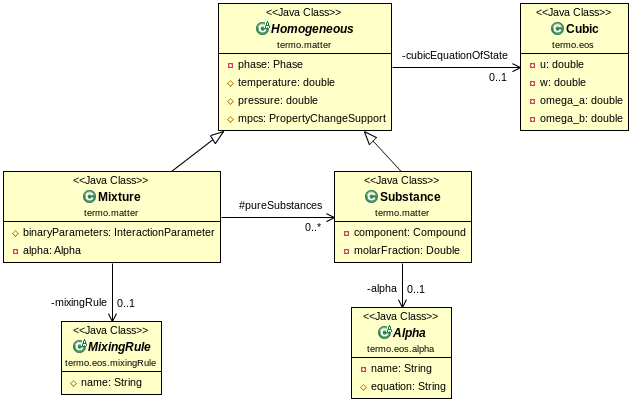
\includegraphics[scale=0.7]{homogeneousCalculations.png}
    \caption{Estructura de la librería para el cálculo de propiedades.}
    \label{fig:homogeneousCalculations}
\end{figure}

Nótese de la figura \ref{fig:homogeneousCalculations} los siguiente:
\begin{itemize}
	\item Que la clase `Homogeneous' contiene una ecuación del tipo `Cubic'.
 	\item Que las clases `Substance' y `Mixture' heredan las propiedades de la clase `Homogenous', como la ecuación cúbica, y puede hacer uso de ella.

\end{itemize}

	Cualquiera de las dos implementaciones de la clase `Homogeneous' tiene los métodos necesarios para calcular los parámetros de la ecuación cúbica según el código \ref{lst:homogeneousParameters}.

\begin{lstlisting}[caption=Cualquier objeto tipo `Homogeneous' puede calcular los parámetros de la ecuación de estado cúbica a y b, label={lst:homogeneousParameters}]
	Homogeneous homogeneous = ...// Objeto tipo `Homogeneous'.
	double a = homogeneous.calculate_a_cubicParameter();
	double b = homogeneous.calculate_b_cubicParameter();
\end{lstlisting}


\subsection{Compuesto puro}\label{subsec:substance}

Como se muestra en la figura \ref{fig:homogeneousCalculations} la clase `Substance' continene una expresión de $\alpha$, y una ecuación de estado, necesarias para realizar el cáculo de los parámetros, segun las ecuaciones \ref{eq:a} y \ref{eq:b}. 

La expresión de $\alpha$ puede ser una función de la temperatura, las expresiones implementadas en el presente trabajo se muestran en la tabla \ref{tab:alphas}.

\begin{table}[!h]
	\centering
	\caption{Expresiónes de $\alpha$ disponibles en la librería}\label{tab:alphas}
	\begin{tabular}{|c|c|c| }
		\hline
		Expresión & Parámetros & Ecuación de estado\\
		\hline
		Soave    &  ---& PR\\
		Peng and Robinson & ---& PR \\
		Mathias & $A$ & SRK\\
		Stryjek and Vera & $k_1$ & PRSV\\
		Adachi and Lu & $A,B$&SRK,PR\\
		Soave & $A,B$&SRK,PR\\
		Melhem, et al. & $A,B$&SRK,PR\\
		Androulakis et al. & $A,B,C$& SRK,PR\\
		Mathias and Copeman & $A,B,C$& SRK,PR\\
		Yu and Lu & $A,B,C$&SRK,PR\\
		Stryjek and Vera & $A,B,C$&PR\\
		Twu & $L,M,N$&TST\\
		Twu & ---&TST,PR\\
		GCEOS & ---& (Cualquier u y w)\\
		\hline
	\end{tabular}
\end{table}
\subsubsection{Creación de un objeto tipo `Substance'}\label{subsub:substanceCreation}

Es necesario utilizar el método constructor de la clase `Substance' para crear un objeto de este tipo, se debe proporcionar como parámetros la ecuación de estado deseada, la exprsión de $\alpha$, una instancia de la clase `Compound' como se muestra en la sección \ref{sec:compounds} y la fase de la substancia.

En la sección \ref{subsec:cubicCreation} se mostró como crear una ecuación de estado cúbica previamente definida, a través de la clase `EquatiosOfState'. Los valore de $\Omega_a$ y $\Omega_b$ se muestran en la tabla \ref{tab:cubics}. De forma muy similar al de las ecuaciońes de estado,la selección de la expresión de $\alpha$ se realiza a través de la clase `Alphas'.

El código \ref{lst:substanceCreation} muestra como crear una objeto del tipo substancia.

\begin{lstlisting}[caption={Creación de un objeto tipo `Substance' para el compuesto Ciclohexano, con la ecuación de estado Soave Redlich Kwong y la expresión de $\alpha$ de mathias },label={lst:substanceCreation}]

Compound compound = new Compound("Cyclohexane");
compound.setCriticalPressure(4073000);
compound.setCriticalTemperature(553.5);
compound.setAcentricFactor(0.211);


Cubic srk = EquationsOfState.redlichKwongSoave();
Alpha mathias = Alphas.getMathiasExpression();


Substance substance = new Substance(srk,mathias, compound,Phase.LIQUID);
\end{lstlisting}

	Finalmente se utiliza el objeto creado para realizar el cálculo de los parámetros de la ecuación de estado cúbica, en el código \ref{lst:substanceParams}.

\begin{lstlisting}[caption={Cálculo de los parámetros para la ecuación de estado cúbica con la clase `Substance'.},label={lst:substanceParams}]
double a = substance.calculate_a_cubicParameter();
double b = substance.calculate_b_cubicParameter();
\end{lstlisting}
 

Nótese que el código \ref{lst:homogeneousParameters} y el código \ref{lst:substanceParams} es idéntico y aunque parece redundate, solo se muestra para señalar el polimorfismo de la librería , es decir que el objeto substance es del tipo `Homogeneous' además del tipo `Substance', y tiene accesso a los métodos en las dos clases.


\subsubsection{Mezcla}\label{subsec:mixture}

El cálculo de los parámetros para una mezcla depende de la regla de mezclado, y en el caso de las reglas de mezclado basadas en la energía libre de exceso, también del modelo de actividad.

Las reglas de mezclado incluidas en este trabajo se muestran en la tabla \ref{tab:mixingrules}, y los modelos de actividad se listan en la tabla \ref{tab:activitymodels}.

\begin{table}[!h]
	\caption{Reglas de mezclado implementadas}\label{tab:mixingrules}
	\begin{tabularx}{\textwidth}{|X|X|X|}
		\hline
		Regla & Parámetros & \\
		\hline
		Van Der Waals & $k_{ij}$ & $k_{ij} = k_{ji}$ \\
		Mathias-Klotz-Prausnitz& $k_{ij}$ & $k_{ij} \neq k_{ji}$ \\
		Huron Vidal & Según el model de actividad & \\
		Wong Sandler & $k_{ij}$ + los parámetros del modelo de actividad & $k_{ij} = k_{ji}$ \\
		\hline
	\end{tabularx}
\end{table}

\begin{table}[!h]
	\caption{Modelos de actividad }\label{tab:activitymodels}
	\begin{tabularx}{\textwidth}{|X|X|X|}
		\hline
		Modelo de actividad & Parámetros & \\
		\hline
		Wilson & $a_{ij}$, $b_{ij}$  & \\
		NRTL & $a_{ij}$, $b_{ij}$, $\alpha_{ij}$ & $\alpha_{ij} = \alpha_{ji}$ \\
		\hline
	\end{tabularx}
\end{table}
\subsubsection{Creación de un objeto tipo `Mixture'}\label{subsub:mixtureCreation}

Un objeto tipo `Mixture' contiene dentro de sí un conjuto de objetos tipo `Substance', esto hace que su creación sea mas compleja. Se ha escrito la clase `MixtureBuilder' para facilitar la creación de los objetos de la clase `Mixture'.

La clase `MixtureBuilder' facilita la creación de los objetos `Substance' que forman el conjunto de compuestos de la mezcla, y permite asignar una expresión de $\alpha$ diferente para cada compuesto.

El código \ref{lst:mixturecreation} muestra la creación de una mezcla, donde la expresión de $\alpha$ es la misma para cada compuesto puro. 

\begin{lstlisting}[caption={Creación de una mezcla con la clase `MixtureBuilder' asignando la misma expresión de $\alpha$ para cada compuesto puro.}, label={lst:mixturecreation} ]

Compound cyclohexane = new Compound("Cyclohexane");
cyclohexane.setCriticalPressure(4073000);
cyclohexane.setCriticalTemperature(553.5);
cyclohexane.setAcentricFactor(0.211);

Compound pentane = new Compound("N-pentane");
pentane.setCriticalPressure(3370000);
pentane.setCriticalTemperature(469.7);
pentane.setAcentricFactor(0.251);

Cubic equationOfState = EquationsOfState.pengRobinson();
Alpha alpha = Alphas.getMathiasAndCopemanExpression();

Mixture mixture = new MixtureBuilder()
			.addCompounds(cyclohexane,pentane)
			.setAlpha(alpha)
			.setEquationOfState(equationOfState)
			.setPhase(Phase.VAPOR)
			.build();

\end{lstlisting}

Es posible crear la mezcla con una expresión de $\alpha$ diferente para cada compuesto puro según el código \ref{lst:mixtureParametersDifAlphas}. 


\begin{lstlisting}[caption={Código para el cálculo de los parámetros de la ecuación de estado en una mezcla, con diferentes expresiones de $\alpha$},label={lst:mixtureParametersDifAlphas}]
Mixture mixture = new MixtureBuilder()
			.addCompound(cyclohexane,Alphas.getPengAndRobinsonExpression())
			.addCompound(pentane,Alphas.getStryjekAndVeraExpression())
			.setEquationOfState(eos)
			.setPhase(phase)
			.setMixingRule(mixingRule)
			.setInteractionParameter(k)
			.build();
\end{lstlisting}

Finalmente se pueden calcular los parámetros de la ecuación cúbica con el código \ref{lst:mixtureParameters}.

\begin{lstlisting}[caption={Cálculo de parámetros de la mezcla},label={lst:mixtureParameters}]
double a = mixture.calculate_a_cubicParameter();
double b = mixture.calculate_b_cubicParameter();
\end{lstlisting}
%hecho

		\section{Materia homogénea}\label{sec:homogeneous}

	La clase `Homogeneous' representa a las substancias o mezclas que se encuentran en una sola fase, las propiedades que se pueden calcular de una fase son: 
\begin{itemize}
	\item fugacidad
	\item presión
	\item factor compresibilidad 
	\item volume molar
	\item entalpía 
	\item entropía 
	\item energía libre de gibbs.
\end
			\subsection{Entalpía}\label{subsec:enthalpy}

	Para conocer la entalpía real de una substacia o mezcla, es necesario conocer la entalpía del gas ideal y la entalpía residual.

\subsubsection{Entalpía del gas ideal}
	Para realizar el cálculo de la entalpía segun el gas ideal, es necesaria una ecuación que represente la capacidad calorífica $C_p$. El cálculo depende de la forma de la ecuación y el valor de sus parámetros. En la sección \ref{sec:cp} se muestran las ecuaciónes de $C_p$ incluidas en la librería.

	Con la ecuación del $C_p$ la clase `Homogeneous' puede calcular la entalpía del gas ideal como se muestra en el código \ref{lst:idealgasenthalpy}.

	\begin{lstlisting}[label={lst:idealgasenthalpy},caption={Cálculo de la entalpía del gas ideal.}]
	double idealGasEnthalpy = homogeneous.calculateIdealGasEnthalpy():
	\end{lstlisting}
	
\subsubsection{Entalpía real}

	La entalpía residual no esta separada en un método particular dentro de la librería \Materia, sino que esta incluido en el cálculo de la entalpía real. Es muy facil realizar la separación, pero para los objetivos de la presente tesis no fue necesario realizarlo.

	El cálculo de la entalpía se realiza en el método `calculateEnthalpy()' como se muestra en el fragmento de código \ref{lst:enthalpy} según la ecuación \ref{eq:enthalpy}. 

\begin{lstlisting}[caption={Cálculo de la entalpía real},label={lst:enthalpy}]
	double enthalpy = homogeneous.calculateEnthapy();
\end{lstlisting}
	
	Las figuras \ref{fig:2denthalpy} y \ref{fig:enthalpy3d} muestran diagramas de entalpía creados con ayuda de la librería \Materia.

\begin{figure}[!h]
	\centering	
	\begin{tikzpicture}
	\begin{axis}[xlabel={\enthalpy},ylabel={\pressure}]
	\addplot[blue]table{plotdata/enthalpy/lv.dat};
	\end{axis}
	\end{tikzpicture}
	\caption{Diagrama de entalpía para el agua. Las líneas azules representan isotermas. }\label{fig:2denthalpy}
\end{figure}


%\addplot+[point meta=explicit]table[x=xcolname,y=ycolname,meta=colordata]{datafile.dat};%ejemplo de uso meta
\begin{figure}[!h]
%\begin{tabular}{c c}
	\begin{tikzpicture}
		\begin{axis}[view/h=-165,
					xlabel={\enthalpy},
					ylabel={\molarVolume},
					zlabel={\pressure},
					colorbar,
					colorbar style={ylabel=Temperatura (K),
					 							title=Código de color}
					]
			\addplot3[surf,point meta=explicit]table[meta=temperature]{plotdata/enthalpy/lv3d.dat};
			\addplot3[surf,point meta=explicit]table[meta=temperature]{plotdata/enthalpy/l3d.dat};
			\addplot3[surf,point meta=explicit]table[meta=temperature]{plotdata/enthalpy/v3d.dat};
		\end{axis}
	\end{tikzpicture}
	%&
% 	\begin{tikzpicture}
% 	\begin{axis}[view/h=-225,xlabel={\enthalpy},ylabel={\molarVolume},zlabel={\pressure}]
% 	\addplot3[surf,point meta=explicit]table[meta=temperature]{plotdata/enthalpy/lv3d.dat};
% 	\addplot3[surf,point meta=explicit]table[meta=temperature]{plotdata/enthalpy/l3d.dat};
% 	\addplot3[surf,point meta=explicit]table[meta=temperature]{plotdata/enthalpy/v3d.dat};
% 	\end{axis}
% 	\end{tikzpicture}
% %\\
%  %\multicolumn{2}{|c|}{
% 	\begin{tikzpicture}
% 	\begin{axis}[view/h=-120,xlabel={\enthalpy},ylabel={\molarVolume},zlabel={\pressure}]
% 	\addplot3[surf,point meta=explicit]table[meta=temperature]{plotdata/enthalpy/lv3d.dat};
% 	\addplot3[surf,point meta=explicit]table[meta=temperature]{plotdata/enthalpy/l3d.dat};
% 	\addplot3[surf,point meta=explicit]table[meta=temperature]{plotdata/enthalpy/v3d.dat};
% 	\end{axis}
% 	\end{tikzpicture}
%}
	\caption{Diagrama tridimensional presión-entalpía-`volumen molar' del agua.}
	\label{fig:enthalpy3d}

%\end{tabular}
\end{figure}	
			\subsection{Entropía}

	El cálculo de la entropía es muy semejante al de la entalpía, es necesario conocer la entropía del gas ideal y la entropía residual.

\subsubsection{Entropía del gas ideal con la ecuación del calor específico}

	El cálculo de la entropía segun el gas ideal, también necesita una ecuación que represente el calor específico. En la sección \ref{sec:cp} se muestran las ecuaciónes de cp incluidas en la librería y como usarlas.

	En el fragmento de código \ref{lst:idealgasentropy} se muestra el cálculo de la entropía del gas ideal según la ecuación \ref{eq:idealgasentropy}. 

	\begin{lstlisting}[label={lst:idealgasentropy},caption={Cálculo de la entropía absoluta del gas ideal.}]
	double idealGasEntropy = homogeneous.calculateIdealGasEntropy();
	\end{lstlisting}

\subsubsection{Entropía real}

	El cálculo de la entalpía se realiza según la ecuación \ref{eq:entropy} y su uso se muestra en el código \ref{lst:entropy}.

\begin{lstlisting}[label={lst:entropy},caption={Cálculo de la entropía absoluta.}]
	double entropy = homogeneous.calculateEntropy()
\end{lstlisting}

	Las figuras \ref{fig:2dentropy} y \ref{fig:entropy3d} muestran diagramas de entalpía creados con ayuda de la librería \Materia.


\begin{figure}[!h]
	\centering	
	\begin{tikzpicture}
	\begin{axis}[xlabel={\entropy},ylabel=\pressure]
	\addplot[blue]table{plotdata/entropy/lv.dat};
	\end{axis}
	\end{tikzpicture}
	\caption{Diagrama de presión-entropía para el agua.}\label{fig:2dentropy}
\end{figure}


%	\begin{tikzpicture}
%	\begin{axis}[view/h=-45,xlabel={\entropy},ylabel={\molarVolume},zlabel={\pressure},colorbar]
%	\addplot3[surf,point meta=explicit]table[meta=temperature,x=pressure,y=entropy,z=temperature]{plotdata/entropy/lv3d.dat};
%	\addplot3[surf,point meta=explicit]table[meta=temperature,x=pressure,y=entropy,z=temperature]{plotdata/entropy/l3d.dat};
%	\addplot3[surf,point meta=explicit]table[meta=temperature,x=pressure,y=entropy,z=temperature]{plotdata/entropy/v3d.dat};
%	\end{axis}
%	\end{tikzpicture}

\begin{figure}[!h]
	\begin{tikzpicture}
	\begin{axis}[view/h=-165,xlabel={\entropy},ylabel={\molarVolume},zlabel={\pressure},colorbar]
	\addplot3[surf,point meta=explicit]table[meta=temperature]{plotdata/entropy/lv3d.dat};
	\addplot3[surf,point meta=explicit]table[meta=temperature]{plotdata/entropy/l3d.dat};
	\addplot3[surf,point meta=explicit]table[meta=temperature]{plotdata/entropy/v3d.dat};
	\end{axis}
	\end{tikzpicture}
	\begin{tikzpicture}
	\begin{axis}[view/h=-225,xlabel={\entropy},ylabel={\molarVolume},zlabel={\pressure}]
	\addplot3[surf,point meta=explicit]table[meta=temperature]{plotdata/entropy/lv3d.dat};
	\addplot3[surf,point meta=explicit]table[meta=temperature]{plotdata/entropy/l3d.dat};
	\addplot3[surf,point meta=explicit]table[meta=temperature]{plotdata/entropy/v3d.dat};
	\end{axis}
	\end{tikzpicture}
	\begin{tikzpicture}
	\begin{axis}[view/h=-120,xlabel={\entropy},ylabel={\molarVolume},zlabel={\pressure}]
	\addplot3[surf,point meta=explicit]table[meta=temperature]{plotdata/entropy/lv3d.dat};
	\addplot3[surf,point meta=explicit]table[meta=temperature]{plotdata/entropy/l3d.dat};
	\addplot3[surf,point meta=explicit]table[meta=temperature]{plotdata/entropy/v3d.dat};
	\end{axis}
	\end{tikzpicture}
	\caption{Diagramas tridimensionales presión-entropía-`volumen molar' para el agua.}\label{fig:entropy3d}
\end{figure}
			\subsection{Energía libre de Gibbs}
	
	El cálculo de la energía libre de Gibbs se realiza a partir de la entropía y la entalpía segun la ecuación \ref{eq:gibbs} y su cálculo se demuestra en el código \ref{lst:gibbs}.

	\begin{lstlisting}[label={lst:gibbs},caption={Cálculo de la energía libre de Gibbs con la librería \Materia}]
		double gibbs = homogeneous.calculateGibbs();
	\end{lstlisting}

	Las figuras \ref{fig:2dgibbs} y \ref{fig:gibbs3d} muestran diagramas de entalpía creados con ayuda de la librería \Materia.

\begin{figure}[!h]
	\centering	
	\begin{tikzpicture}
	\begin{axis}
	\addplot[blue]table{plotdata/gibbs/lv.dat};
	\end{axis}
	\end{tikzpicture}
	\caption{Diagrama de la energía libre de Gibbs para el agua.}\label{fig:2dgibbs}
\end{figure}

\begin{figure}[!h]
	\begin{tikzpicture}
	\begin{axis}[view/h=-165,xlabel={\gibbs},ylabel={\molarVolume},zlabel={\pressure},colorbar]
	\addplot3[surf,point meta=explicit]table[meta=temperature]{plotdata/gibbs/lv3d.dat};
	\addplot3[surf,point meta=explicit]table[meta=temperature]{plotdata/gibbs/l3d.dat};
	\addplot3[surf,point meta=explicit]table[meta=temperature]{plotdata/gibbs/v3d.dat};
	\end{axis}
	\end{tikzpicture}
	\begin{tikzpicture}
	\begin{axis}[view/h=-225,xlabel={\gibbs},ylabel={\molarVolume},zlabel={\pressure}]
	\addplot3[surf,point meta=explicit]table[meta=temperature]{plotdata/gibbs/lv3d.dat};
	\addplot3[surf,point meta=explicit]table[meta=temperature]{plotdata/gibbs/l3d.dat};
	\addplot3[surf,point meta=explicit]table[meta=temperature]{plotdata/gibbs/v3d.dat};
	\end{axis}
	\end{tikzpicture}
	\begin{tikzpicture}
	\begin{axis}[view/h=-120,xlabel={\gibbs},ylabel={\molarVolume},zlabel={\pressure}]
	\addplot3[surf,point meta=explicit]table[meta=temperature]{plotdata/gibbs/lv3d.dat};
	\addplot3[surf,point meta=explicit]table[meta=temperature]{plotdata/gibbs/l3d.dat};
	\addplot3[surf,point meta=explicit]table[meta=temperature]{plotdata/gibbs/v3d.dat};
	\end{axis}
	\end{tikzpicture}
	\caption{Diagramas tridimensionales de presión-`energía libre de Gibbs'-`volumen molar' para el agua.}\label{fig:gibbs3d}
\end{figure}
			 \subsection{Presión}\label{subsec:pressure}
	Un cálculo de presión, se realiza como se muestra en el código \ref{lst:pressureCalculation}.
	\begin{lstlisting}[label=lst:pressureCalculation,caption=Cálculo de presión para un objeto tipo homogeneous]
	double pressure = homogeneous.calculatePressure(temperature, volume);
	\end{lstlisting}

	Como ya se mencionó antes el objeto `Homogeneous' del código \ref{lst:pressureCalculation} puede ser una substancia o una mezcla.

 	En la figura \ref{fig:cubicPressureDiagrams} se muestra un ejemplo de uso del cálculo para realizár gŕaficas de presión.

	\begin{figure}[!h]
	\begin{tabular}{c c}
		\begin{tikzpicture}
		\begin{axis}[width= 0.45 \linewidth,font=\footnotesize,
		xlabel = {Volumen molar $[\frac{m^3}{kmol}]$},
		ylabel = {Presión $[Pa]$}]
		\addplot[blue]table{plotdata/pressurevolume.dat};
		\end{axis}
		\end{tikzpicture}
		&
		\begin{tikzpicture}
		\begin{axis}[width= 0.45 \linewidth,,font=\footnotesize,
		xlabel={Volumen molar $[\frac{m^3}{kmol}]$},
		zlabel={Presión $[Pa]$},
		ylabel={Temperatura $[K]$}]
		\addplot3[surf,
		colormap={blueblack}{color=(white) color=(blue)},
		domain=0:1]table{plotdata/pressurevolumetemperature.dat};
		\end{axis}
		\end{tikzpicture}
	\end{tabular}
	\caption{Diagramas de presión para el heptano usando la eq. de Van Der Waals (u=w=0)} \label{fig:cubicPressureDiagrams}
	\end{figure}


	

			\subsection{Factor de compresibilidad}\label{subsec:compresibilityFactor}

Es necesario realizar la solución de la ecuación de estado cúbica para conocer el factor de compresibilidad. La solución de la ecuación se realiza en el método ``calculateCompresibilityFactor'' de la clase ``Cubic''.

El método recibe los parámetros adimensionales A, B y la fase a la cual se desea calcular el factor de compresibilidad. La clase ``Cubic'' tiene los métodos necesarios para transformar los parámetros a y b a su forma adimensional A y B.

El el fragmento de código \ref{lst:compresibility} se muestra la creación de la ecuación de estado cúbica, adimensionalización de los parámetros y finalmente el cálculo de el factor de compresibilidad.

\begin{lstlisting}[label=lst:compresibility,caption={Cálculo del factor de compresibilidad, y adimensionamiento de los parámetros a y b con la clase ``Cubic''}]
Cubic cubic = EquationsOfState.vanDerWaals();
		
double criticalTemperature = 540.2;
double criticalPressure = 2.74000E+06;

double pressure = criticalPressure * 1.5;
double reducedTemperature= criticalTemperature * 2;

//parametros de van Der Waals para el heptano
double a = 3107000.0;
double b = 0.2049;

double A =cubic.get_A(temperature, pressure, a);
double B = cubic.get_B(temperature, pressure, b);

double z =cubic.calculateCompresibilityFactor(A, B, Phase.LIQUID);
\end{lstlisting}
 
	Gracias a esta librería podemos formar los diagramas de la figura \ref{fig:zchart}.

\begin{figure}
\begin{tabular}{c c}
	\begin{tikzpicture}
	\begin{axis}[width=0.45\linewidth,font=\footnotesize,view/v=-6,
		ylabel= {Presión reducida },
		xlabel= {Temperatura reducida},
		zlabel={Factor de compresibilidad z}]%[colormap/hot]
	\addplot3[surf,point meta=explicit] table[meta=rt,x=p,y=rt,z=z]{plotdata/compresibilitiChart/pz_temp.dat};
	\end{axis}
	\end{tikzpicture}
	&
	\begin{tikzpicture}
	\begin{axis}[width=0.45\linewidth,font=\footnotesize,
		xlabel= {Presión reducida },
		ylabel= {Factor de compresibilidad z}]%[colormap/hot]
	\addplot[blue]table{plotdata/compresibilitiChart/pz_temp.dat};
	\end{axis}
	\end{tikzpicture}
\end{tabular}
\caption{Diagramas del factor de compresibilidad }
\label{fig:zchart}
\end{figure}
%hecho
			\subsection{Volumen molar}\label{subsec:volume}
	
	El código \ref{lst:volume} muestra como calcular el volumen molar para una substancia o mezcla homogénea.  

\begin{lstlisting}[label={lst:volume},caption={Cálculo del factor de double volume = cubic.}]
	double volume = calculateVolume(temperature, pressure, z);
\end{lstlisting}
	
	En la figura \ref{fig:volume} se muestra la relación que tiene el volumen con el factor de compresibilidad a diferentes temperaturas y presiones.

\begin{figure}[!h]
\begin{tabular}{c c}
	\begin{tikzpicture}
	\begin{axis}[width=0.45\linewidth,font=\footnotesize,view/h=-195,
		ylabel= {Volumen reducido},
		xlabel= {Presión reducida},
		zlabel={Factor de compresibilidad z}]%[colormap/hot]
	\addplot3[surf,point meta=explicit] table[meta=rt,x=p,y=vr,z=z]{plotdata/volume/pz_vr.dat};
	\end{axis}
	\end{tikzpicture}
	&
	\begin{tikzpicture}
	\begin{axis}[width=0.45\linewidth,font=\footnotesize,view/h=90,view/v=-0,
		ylabel= {Volumen reducido},
		zlabel={Factor de compresibilidad z}]%[colormap/hot]
	\addplot3[surf,point meta=explicit] table[meta=rt,x=p,y=vr,z=z]{plotdata/volume/pz_vr.dat};
	\end{axis}
	\end{tikzpicture}
\end{tabular}
\caption{Relación entre el factor de compresibilidad y el volumen}\label{fig:volume}
\end{figure}%hecho
			\subsection{Fugacidad}\label{subsec:fugacity}

\begin{multline}
\ln\hat{\phi_i} = - \ln\left(\frac{v-b}{v}\right) 
+ (z-1)\left[\frac{1}{b}\frac{\partial bN}{\partial N_i}\right]
+ \frac{a}{RTb\sqrt{u^2-4w}}
\\
\left[\frac{1}{b}\frac{\partial bN}{\partial N_i}
- \frac{1}{aN}\frac{\partial aN²}{\partial N_i}\right]
\ln\left[\frac{2v+b\left(u + \sqrt{u²-4w}\right)}{2v+b\left(u - \sqrt{u²-4w}\right)}\right]
-\ln{z}
\end{multline}  
		
		\section{Equilibrio Líquido-Vapor}\label{sec:heterogeneous}
		\subsection{Temperatura de Burbuja}\label{subsec:bubbletemperature}

	El cálculo de temperatura de burbuja para una mezcla se realiza como se indica en la figura \ref{fig:bubbletemperature}. Usando un objeto del tipo `HeterogeneousMixture' de la librería \Materia el cálculo se realiza como se muestra en los fragmentos de código \ref{lst:bubbletemperature} y \ref{lst:bubbletemperatureWithEstimate}.

	Si al método no se le proporciona un estimado inicial, como se muestra en el código \ref{lst:bubbletemperature} entonces la clase realiza la estimación de la temperatura como se muestra en la figura \ref{fig:bubbletemperatureEstimate}. 

	\begin{lstlisting}[label={lst:bubbletemperatureWithEstimate},caption={Cálculo de la temperatura de burbuja proporcionando un estimado inicial.}]

		heterogeneousMixture.setZFraction(compound1,molarFraction1);
		//...... asignar la fracción molar para todos los compuestos

		heterogeneousMixture.setPressure(pressure);
		heterogeneousMixture.bubbleTemperature(temeperatureEstimate);
		double temperature = heterogeneousMixture.getTemperature();
	\end{lstlisting}


	\begin{lstlisting}[label={lst:bubbletemperature},caption={Cálculo de la temperatura de burbuja.}]

		heterogeneousMixture.setZFraction(compound1,molarFraction1);
		//...... asignar la fracción molar para todos los compuestos

		heterogeneousMixture.setPressure(pressure);
		heterogeneousMixture.bubbleTemperature();
		double temperature = heterogeneousMixture.getTemperature();
	\end{lstlisting}



		\subsection{Temperatura de Rocío}\label{subsec:dewtemperature}

	El cálculo de temperatura de rocío para una mezcla se realiza como se indica en la figura \ref{fig:dewtemperature}. Usando un objeto del tipo `HeterogeneousMixture' de la librería \Materia el cálculo se realiza como se muestra en los fragmentos de código \ref{lst:dewtemperature} y \ref{lst:dewtemperatureWithEstimate}.

	Si al método no se le proporciona un estimado inicial, como se muestra en el código \ref{lst:dewtemperature} entonces la clase realiza la estimación de la temperatura como se muestra en la figura \ref{fig:dewtemperatureEstimate}. 

	\begin{lstlisting}[label={lst:dewtemperatureWithEstimate},caption={Cálculo de la temperatura de rocío proporcionando un estimado inicial.}]

		heterogeneousMixture.setZFraction(compound1,molarFraction1);
		//...... asignar la fracción molar para todos los compuestos

		heterogeneousMixture.setPressure(pressure);
		heterogeneousMixture.dewTemperature(
			temeperatureEstimate,liquidEstimatedFractions);
		double temperature = heterogeneousMixture.getTemperature();
	\end{lstlisting}


	\begin{lstlisting}[label={lst:dewtemperature},caption={Cálculo de la temperatura de rocío.}]

		heterogeneousMixture.setZFraction(compound1,molarFraction1);
		//...... asignar la fracción molar para todos los compuestos

		heterogeneousMixture.setPressure(pressure);
		heterogeneousMixture.dewTemperature();
		double temperature = heterogeneousMixture.getTemperature();
	\end{lstlisting}


		\subsection{Presión de Burbuja}\label{subsec:bubblepressure}

	El cálculo de presión de burbuja para una mezcla se realiza como se indica en la figura \ref{fig:bubblepressure}. Usando un objeto del tipo `HeterogeneousMixture' de la librería \Materia el cálculo se realiza como se muestra en los fragmentos de código \ref{lst:bubblepressure} y \ref{lst:bubblepressureWithEstimate}.

	Si al método no se le proporciona un estimado inicial, como se muestra en el código \ref{lst:bubblepressure} entonces la clase realiza la estimación de la presión de vapor con la ecuación del factor acéntrico \ref{eq:pressureacentricfactor}. 



	\begin{lstlisting}[label={lst:bubblepressureWithEstimate},caption={Cálculo de la presión de burbuja proporcionando un estimado inicial.}]

		heterogeneousMixture.setZFraction(compound1,molarFraction1);
		//...... asignar la fracción molar para todos los compuestos

		heterogeneousMixture.setTemperature(temperature);
		heterogeneousMixture.bubblePressure(pressureEstimate);
		double pressure = heterogeneousMixture.getPressure();
	\end{lstlisting}


	\begin{lstlisting}[label={lst:bubblepressure},caption={Cálculo de la presión de burbuja.}]
		heterogeneousMixture.setZFraction(compound1,molarFraction1);
		//...... asignar la fracción molar para todos los compuestos

		heterogeneousMixture.setTemperature(temperature);
		heterogeneousMixture.bubblePressure();
		double pressure = heterogeneousMixture.getPressure();
	\end{lstlisting}

	La figura \ref{fig:bubblepressure3d} muestra el resultado del cálculo de presión de burbuja para el sistema metanol-agua.

\begin{figure}[p]
\centering
	\begin{tikzpicture}
	\begin{axis}[view/v=-15,colorbar left,xlabel={Fracción Molar del metanol},ylabel=\temperature,zlabel=\pressure,colorbar style={ylabel=\temperature,
        yticklabel style={
            text width=2.5em,
            align=right}}]
		\addplot3[surf,point meta=explicit,shader=interp]table[meta=temperature, y=temperature , x=liquidFraction, z=pressure]{plotdata/mixhet/hp.dat};
		\addplot3[surf,point meta=explicit,shader=interp]table[meta=temperature, y=temperature , x=vaporFraction, z=pressure]{plotdata/mixhet/hp.dat};
	\end{axis}
	\end{tikzpicture}


	\begin{tikzpicture}
	\begin{axis}[view/v=-220,xlabel={Fracción Molar del metanol},ylabel=\temperature,zlabel=\pressure]
	\addplot3[surf,point meta=explicit,shader=interp]table[meta=temperature, y=temperature , x=liquidFraction, z=pressure]{plotdata/mixhet/hp.dat};
	\addplot3[surf,point meta=explicit,shader=interp]table[meta=temperature, y=temperature , x=vaporFraction, z=pressure]{plotdata/mixhet/hp.dat};
	\end{axis}
	\end{tikzpicture}


	\begin{tikzpicture}
	\begin{axis}[view/v=-115,xlabel={Fracción Molar del metanol},ylabel=\temperature,zlabel=\pressure]
	\addplot3[surf,point meta=explicit,shader=interp]table[meta=temperature, y=temperature , x=liquidFraction, z=pressure]{plotdata/mixhet/hp.dat};
	\addplot3[surf,point meta=explicit,shader=interp]table[meta=temperature, y=temperature , x=vaporFraction, z=pressure]{plotdata/mixhet/hp.dat};
	\end{axis}
	\end{tikzpicture}
	\caption{Diagramas tridimensionales de presión-composición-temperatura para el sistema metanol-agua. En la figura podemos observar los planos formados por los puntos de burbuja y los puntos de rocío. Los diagramas son la misma figura vista desde diferentes angulos}\label{fig:bubblepressure3d}
\end{figure}

		\subsection{Presión de Rocío}\label{subsec:dewpressure}

	El cálculo de presión de rocío para una mezcla se realiza como se indica en la figura \ref{fig:dewpressure}. Usando un objeto del tipo `HeterogeneousMixture' de la librería \Materia el cálculo se realiza como se muestra en los fragmentos de código \ref{lst:dewpressure} y \ref{lst:dewpressureWithEstimate}.

	Si al método no se le proporciona un estimado inicial, como se muestra en el código \ref{lst:dewpressure} entonces la clase realiza la estimación de la presión de vapor con la ecuación del factor acéntrico \ref{eq:pressureacentricfactor}. 

	\begin{lstlisting}[label={lst:dewpressureWithEstimate},caption={Cálculo de la presión de rocío proporcionando un estimado inicial.}]

		heterogeneousMixture.setZFraction(compound1,molarFraction1);
		//...... asignar la fracción molar para todos los compuestos

		heterogeneousMixture.setTemperature(temperature);
		heterogeneousMixture.dewPressure(pressureEstimate);
		double pressure = heterogeneousMixture.getPressure();
	\end{lstlisting}

	\begin{lstlisting}[label={lst:dewpressure},caption={Cálculo de la presión de rocío.}]

		heterogeneousMixture.setZFraction(compound1,molarFraction1);
		//...... asignar la fracción molar para todos los compuestos

		heterogeneousMixture.setTemperature(temperature);
		heterogeneousMixture.dewPressure();
		double pressure = heterogeneousMixture.getPressure();
	\end{lstlisting}

\begin{figure}[!h]
	\begin{tikzpicture}[nodes={draw, fill=white,align=center},row sep=0.3cm,column sep=0.5cm] ]

	\node(init){Inicio};
	\node[below of=init,below] (lab)  {Lectura de \textbf{Datos} \\$T,y_1, y_2,\ldots, y_{nc}$};
	\node[below of=lab,below=0.4](estim){Estimado inicial de\\ las incognitas\\$P,x_1,x_2,\ldots,x_{nc}$};
	\node[below of=estim,below=0.4](relations){Cálculo de las\\ razones de equilibrio\\
	$K_i = \frac{ \hat{\phi}_i^L }{ \hat{ \phi}_i^V}$};
	\node[below of=relations,below = 0.5cm](error){Cálculo de la función Error\\
	$ S_x =\sum_{i=1}^{nc}\frac{y_i}{ K_i} $\\$ E = S_x-1 $};

	\node[below of=error,below=0.4](criteria){$|E| \leq 1\cdot10^{-4}\quad \text{o} \quad  1\cdot 10^{-5}$};
	\node[below of=criteria,below=0.4](tempIncrement){Incrementer la temperatura\\$P^* = P + \Delta P$\\
	$\Delta P = 0.001  \quad \text{o} \quad 0.0001 K$};

	\node[below of=tempIncrement,below=0.4](relationsWithIncrement){Cálculo de las Razones\\ de Equilibrio con $P^*$\\$K_i^* = \frac{ \hat{\phi}_i^L }{\hat{\phi}_i^V}$};

	\node[right of=criteria	,right=2.2cm](end){Fin};


	\node[right of=tempIncrement, right=3cm](errorWithIncrement){Cálculo de la función Error \\ con $P^*$\\
	$ S_x^* =\sum_{i=1}^{nc} \frac{y_i}{K_i^*}  $\\$ E^* = S_x^*-1 $};

	\node[right of=relations, right = 3cm](newValues){Cálculo de las nuevas estimaciones \\ de las \textbf{Incógnitas}\\
	\begin{minipage}{0.2\linewidth}
	\begin{equation*}
	T_{nueva} =P- \frac{E  \left(P^*-P\right)}{E^*-E}
	\end{equation*}
	\begin{equation*}
	 S_x =\sum_{i=1}^{nc}\frac{y_i}{K_i}   \\
	 \end{equation*}
	 \begin{equation*}
	\left(x_i\right)_{nueva} = \frac{y_i}{K_i S_x}
	\end{equation*}
	\end{minipage}
	};


	\draw[-latex] (init)--(lab);
	\draw[-latex] (lab)--(estim);
	\draw[-latex] (estim)--(relations);
	\draw[-latex] (relations)--(error);
	\draw[-latex] (error)--(criteria);
	\draw[-latex] (criteria)--node[fill=none,draw=none,above]{SI}(end);
	\draw[-latex] (criteria)--node[fill=none,draw=none,left]{NO}(tempIncrement);
	\draw[-latex] (tempIncrement)--(relationsWithIncrement);
	\draw[-latex] (relationsWithIncrement)--(errorWithIncrement);
	\draw[-latex] (errorWithIncrement)--(newValues);
	\draw[-latex] (newValues)--(relations);

	\end{tikzpicture}
	\caption{Algoritmo para el cálculo de la presión de rocío.}\label{fig:dewpressure}
\end{figure}
		\subsection{Flash}\label{subsec:flash}


	El cálculo del flash temperatura-presión se realiza como se indica en la figura \ref{fig:flash}. Usando un objeto del tipo `HeterogeneousMixture' de la librería \Materia el cálculo se realiza como se muestra en el fragmento de código \ref{lst:flash} .

\begin{lstlisting}[label={lst:flash},caption={Cálculo del flash temperatura-presión.}]

	//asignar la fraccion molar para todos los compuestos
	heterogeneousMixture.setZFraction(compound1,molarFraction1);
	//...... 

	double vF = heterogeneousMixture.flash(temperature,pressure);

	//leer las fracciones del vapor y del liquido para todos los compuestos
	double x1 = heterogeneousMixture.getLiquid()
					.getReadOnlyFractions().get(compound1);
	double y1 = heterogeneousMixture.getVapor()
					.getReadOnlyFractions().get(compound1);
	//.....
\end{lstlisting}

\begin{figure}[!h]
	\begin{tikzpicture}[nodes={draw, fill=white,align=center},row sep=0.3cm,column sep=0.5cm] ]

	\node(init){Inicio};
	\node[below of=init,below] (lab)  {Lectura de \textbf{Datos} \\$T,P,z_1, z_2,\ldots, z_{nc}$};
	\node[below of=lab,below=0.4](estim){Estimado inicial de\\ las incognitas\\$V/F,x_1,x_2,\ldots,x_{nc}$\\$y_1,y_2 \ldots, y_{nc}$};
	\node[below of=estim,below=0.4](relations){Cálculo de las\\ razones de equilibrio\\
	$K_i = \frac{ \hat{\phi}_i^L }{ \hat{ \phi}_i^V}$};
	\node[below of=relations,below = 0.4cm](error){Cálculo de la función Error\\
	$ \zeta =\sum_{i=1}^{nc}\left| x_i \hat{\varphi}_i^L - y_i \hat{\varphi}_i^V \right|$};

	\node[below of=error,below=0.4](criteria){$|\zeta| \leq 1\cdot10^{-4}\quad \text{o} \quad  1\cdot 10^{-5}$};


	\node[below of=criteria,below=0.4](rachford){Cálculo de $V/F$ con Rachford-Rice:\\ 
	\begin{minipage}{0.5\linewidth}
	\begin{equation*}
	S = \sum_{i=1}^{nc}\frac{z_i\left(K_i - 1\right)}{1+ \frac{V}{F}\left(K_i-1\right)}
	\end{equation*}
	Encontrar $V/F$ tal que $S = 0$\\
	Método de Newton-Raphson\\
	\begin{equation*}
	\acute{S} = \sum_{i=1}^{nc} \frac{-z_i \left(K_i - 1\right)^2}{\left[1+ \frac{V}{F} \left(K_i-1\right)\right]^2}
	\end{equation*}
	\begin{equation*}
	\left(\frac{V}{F}\right)_{nueva} = \left(\frac{V}{F}\right) - \frac{S}{\acute{S}}
	\end{equation*}
	\end{minipage}};

	\node[right of=criteria	,right=2.2cm](end){Fin};


	\node[right of=estim, right = 3cm](newValues){Cálculo de las nuevas estimaciones \\ de las \textbf{Incógnitas}\\
	\begin{minipage}{0.3\linewidth}
	\begin{equation*}
	\acute{x_i} = \frac{z_i}{1 + \frac{V}{F}\left(K_i-1\right)}
	\end{equation*}
	\begin{equation*}
	 S_x =\sum_{i=1}^{nc}\acute{x}_i \qquad x_i = \frac{\acute{x_i}}{S_x}
	\end{equation*}
	\begin{equation*}
	\acute{y_i} = \acute{x_i} K_i = \frac{z_i K_i}{1+\frac{V}{F}\left(K_i - 1\right)}
	\end{equation*}
	\begin{equation*}
	 S_y =\sum_{i=1}^{nc}\acute{y}_i \qquad y_i = \frac{\acute{y_i}}{S_y}
	\end{equation*}
	\end{minipage}
	};


	\draw[-latex] (init)--(lab);
	\draw[-latex] (lab)--(estim);
	\draw[-latex] (estim)--(relations);
	\draw[-latex] (relations)--(error);
	\draw[-latex] (error)--(criteria);
	\draw[-latex] (criteria)--node[fill=none,draw=none,above]{SI}(end);
	\draw[-latex] (criteria)--node[fill=none,draw=none,left]{NO}(rachford);

	\draw[-latex] (rachford)-|(newValues);
	\draw[-latex] (newValues)--(relations);

	\end{tikzpicture}
	\caption{Algoritmo para el cálculo del flash Temperatura-Presión.}\label{fig:flash}
\end{figure}
		

		\subsection{Diagramas}
	



	\chapter{Optimización de parámetros}
	\section{Parámetros de $\alpha$}

	\section{Parámetros binarios}

\begin{tikzpicture}
\begin{axis}
\addplot[blue,only marks]table[x=temperature, y=exppressure]{plotdata/alphaOptimization/error.dat};
\addplot[red]table[x=temperature,y=calcpressure]{plotdata/alphaOptimization/error.dat};
\end{axis}
\end{tikzpicture}



\begin{tabular}{c c c}
\begin{tikzpicture}
	\begin{axis}
		\addplot[red,only marks]table[x=temperature,y=error]{plotdata/alphaOptimization/error.dat};
		\addplot[blue,only marks]table[x=temperature,y=error]{plotdata/alphaOptimization/minError.dat};
	\end{axis}
\end{tikzpicture}
&
\begin{tikzpicture}
	\begin{axis}[width=5cm]
	\addplot[blue,only marks]table[x=temperature,y=error]{plotdata/alphaOptimization/minError.dat};
	\end{axis}
\end{tikzpicture}
\end{tabular}





\begin{tikzpicture}
\begin{axis}
\addplot[yellow,only marks]table[x=iteration,y=a]{plotdata/alphaOptimization/trayectory2dimension.dat};
\addplot[green,only marks]table[x=iteration,y=b]{plotdata/alphaOptimization/trayectory2dimension.dat};
\end{axis}
\begin{axis}

\addplot[blue,only marks]table[x=iteration,y=error]{plotdata/alphaOptimization/trayectory2dimension.dat};
\end{axis}
\end{tikzpicture}


\begin{tikzpicture}
\begin{axis}% [view/v=45]
\addplot3[surf]table{plotdata/alphaOptimization/params.dat};
\addplot3[red]table{plotdata/alphaOptimization/trayectory.dat};
\end{axis}
\end{tikzpicture}
	\chapter{Optimización de parámetros $Binarios$}


\definecolor{amber}{rgb}{1.0, 0.49, 0.0}

\newcommand{\binaryDiagram}[1] {
\begin{tikzpicture}
\begin{axis}
\addplot[amber,only marks,mark size = 1pt]table[x=x1, y=expTemp]{#1};
\addplot[blue,only marks,mark size = 1pt]table[x=yExp, y=expTemp]{#1};
\addplot[green,thick] table[x=x1, y=calcTemp]{#1};
\addplot[red,thick] table[x=yCalc, y=calcTemp]{#1};
\end{axis}
\end{tikzpicture}
 }

\binaryDiagram{plotdata/binaryOptim/error.dat}

\binaryDiagram{plotdata/binaryOptim/errorAfterOptim.dat}
	\chapter{Paquetes termodinámicos}
	\section{Estructura de la librería}
	 \subsection{Materia Homogénea}

			\begin{figure}[!h]
			  
			  \centering
			    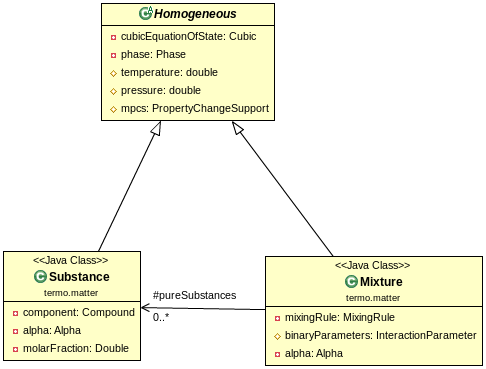
\includegraphics[scale=0.7]{Homogenous.png}
			    \caption{A picture of a gull.}
			\end{figure}

		\subsection{Materia Heterogénea}

			\begin{figure}[!h]
			  
			  \centering
			    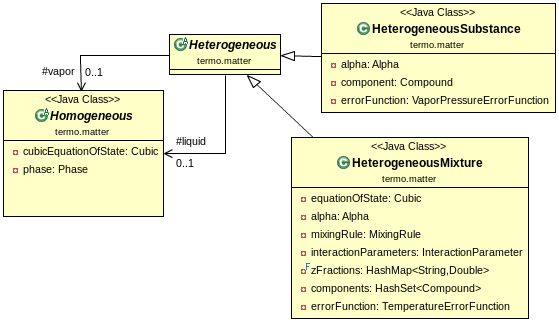
\includegraphics[scale=0.7]{heterogeneous.png}
			    \caption{ads}
			\end{figure}


	
		\subsection{Mezcla}



	\section{Objetos incluidos}
		\subsection{Ecuaciones de estado cúbicas}
		\subsection{Expresiones de $\alpha$}
		\subsection{Reglas de mezclado}
		\subsection{modelos de actividad}
	\section{¿Cómo extender los paquetes?/ ¿Cómo escribir mi propio paquete?}
		\subsection{Fork Repo desde GitHub}
		\subsection{Agregar classes}
		\subsection{Pull Request}

	\chapter{Aplicación de internet}
	\section{Base de datos}
		\subsection{Usuarios}
		\subsection{Componentes}
		\subsection{Listas de datos experimentales}
			\subsubsection{Compuestos}
			\subsubsection{Mezclas}
	
	\include{advancedOptions_chapter}
	\chapter{Diagramas ternarios}

\newcommand{\alphaOptim}[1] {

\begin{tabular}{c c}

\begin{tikzpicture}
	\begin{axis}
		\addplot[blue,only marks,mark size = 1pt]table[x=Temperature,y=experimentalPressure]{plotdata/ternaryDiagram/#1/afterOptim.dat};
		\addplot[red,thick]table[x=Temperature,y=calculatedPressure]{plotdata/ternaryDiagram/#1/afterOptim.dat};
	\end{axis}
\end{tikzpicture}
&
\begin{tikzpicture}
	\begin{axis}
		\addplot[blue,only marks,mark size = 1pt]table[x=Temperature,y=experimentalPressure]{plotdata/ternaryDiagram/#1/beforeOptim.dat};
		\addplot[red,thick]table[x=Temperature,y=calculatedPressure]{plotdata/ternaryDiagram/#1/beforeOptim.dat};
	\end{axis}
\end{tikzpicture}
\\
\begin{tikzpicture}
	\begin{axis}
		\addplot[blue,only marks,mark size = 1pt]table[x=Temperature,y=error]{plotdata/ternaryDiagram/#1/beforeOptim.dat};
		\addplot[red,only marks,mark size = 1pt]table[x=Temperature,y=error]{plotdata/ternaryDiagram/#1/afterOptim.dat};
	\end{axis}
\end{tikzpicture}
&
\begin{tikzpicture}
	\begin{axis}
		\addplot[only marks,mark size = 1pt]table[x=iteration,y=A]{plotdata/ternaryDiagram/#1/history.dat};
		\addplot[only marks,mark size = 1pt]table[x=iteration,y=B]{plotdata/ternaryDiagram/#1/history.dat};
		\addplot[only marks,mark size = 1pt]table[x=iteration,y=C]{plotdata/ternaryDiagram/#1/history.dat};
	
	\end{axis}
\end{tikzpicture}
\\
\begin{tikzpicture}
	\begin{axis}
		\addplot[red,only marks,mark size = 1pt]table[x=iteration,y=Error]{plotdata/ternaryDiagram/#1/history.dat};
	\end{axis}
\end{tikzpicture}
\end{tabular}
}


\newcommand{\binary}[1]{
\begin{tikzpicture}
	\begin{axis}
		\addplot[blue,only marks,mark size = 1pt]table[x=x1,y=pressure]{plotdata/ternaryDiagram/#1/beforeOptim.dat};
		\addplot[red,only marks,mark size = 1pt]table[x=y1,y=pressure]{plotdata/ternaryDiagram/#1/beforeOptim.dat};
		\addplot[green,thick]table[x=y1calc,y=calcpressure]{plotdata/ternaryDiagram/#1/beforeOptim.dat};
		\addplot[brown,thick]table[x=x1,y=calcpressure]{plotdata/ternaryDiagram/#1/beforeOptim.dat};

		\addplot[purple,thick]table[x=y1calc,y=calcpressure]{plotdata/ternaryDiagram/#1/afterOptim.dat};
		\addplot[black,thick]table[x=x1,y=calcpressure]{plotdata/ternaryDiagram/#1/afterOptim.dat};
	\end{axis}
\end{tikzpicture}

}

\alphaOptim{ethylene}
\alphaOptim{water}
\alphaOptim{ethanol}


binary



\binary{ethylenewater}



\begin{tikzpicture}
\begin{ternaryaxis}[xlabel=Agua,
ylabel=Etileno,
zlabel=Etanol]
\addplot3[only marks,blue] table[x=x1,y=x2,z=x3]{plotdata/ternaryDiagram/graph.dat};
\addplot3[only marks,red] table[x=y1,y=y2,z=y3]{plotdata/ternaryDiagram/graph.dat};
\end{ternaryaxis}
\end{tikzpicture}
	\appendix
	\chapter{Ejemplo de uso con Netbeans} \label{}



	\section{Requisitos}

	\begin{enumerate}

	\item Necesitamos tener instalado kit de desarrollo Jdk de java que se puede descargar desde la página (http://www.oracle.com/technetwork/java/javase/downloads/).

	\item Necesitamos tener instalado el ambiente de desarrollo Netbeans que se puede descargar de la página (https://netbeans.org/downloads/).
	\end{enumerate}

	\section{Manualmente}\label{sec:manualInstall}
		Descargar el archivo .jar y agregarlo al folder /lib de la aplicación
		\begin{enumerate}
			\item Desde la página oficial de EQ PRO(ingenieria-eqpro.rhcloud.com) se puede descargar el archivo jar.

			\item Crear un nuevo proyecto desde Netbeans.

			\begin{center}
			  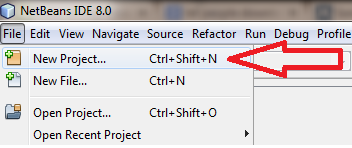
\includegraphics[scale=0.7]{new-proyect.png}
			\end{center}

			\item Elegir el tipo de aplicación java.application 
			\begin{center}
			  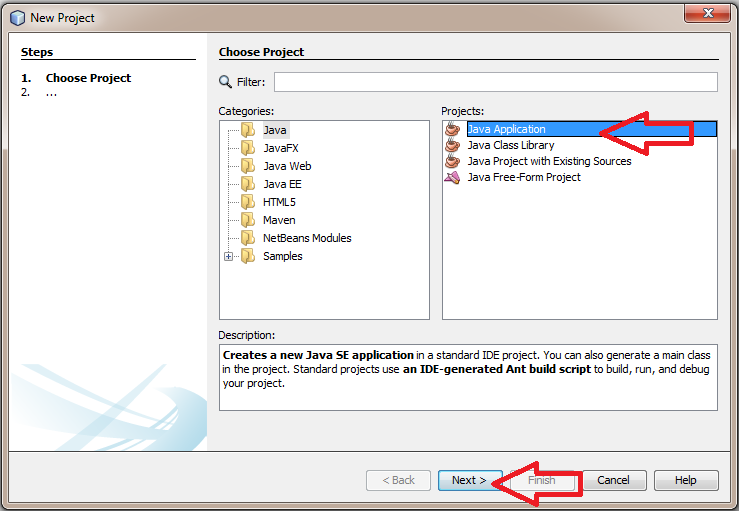
\includegraphics[scale=0.7]{application-type.png} 
			\end{center}
			\item Asignar el nombre del proyecto 
			\begin{center}
			  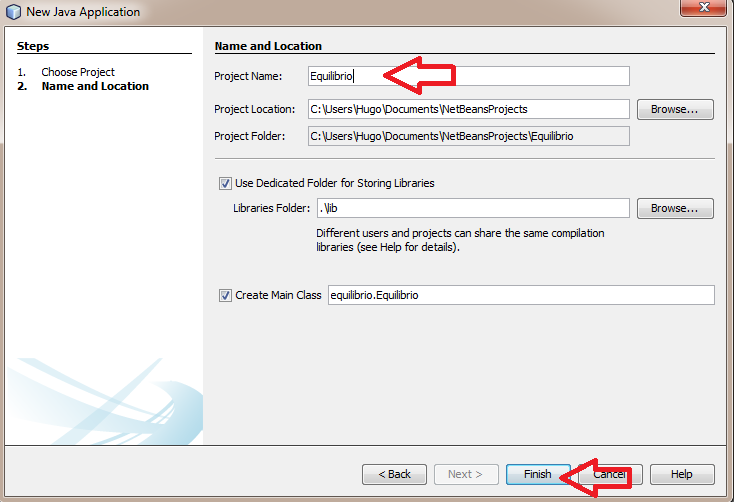
\includegraphics[scale=0.7]{proyect-name.png} 
			\end{center}
			\item En la pestaña proyectos de netbeans, con click derecho en la carpeta “Libraries” elegir la opción “Agregar jar/Folder “.
			\begin{center}
			  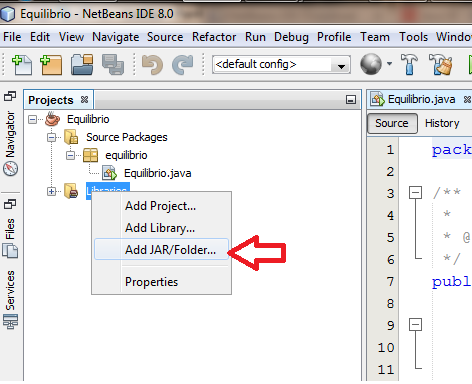
\includegraphics[scale=0.7]{add-jar.png} 
			\end{center}


			 \item Navegar entonces hasta la ruta donde se descargo el archivo jar. 

			\begin{center}
			  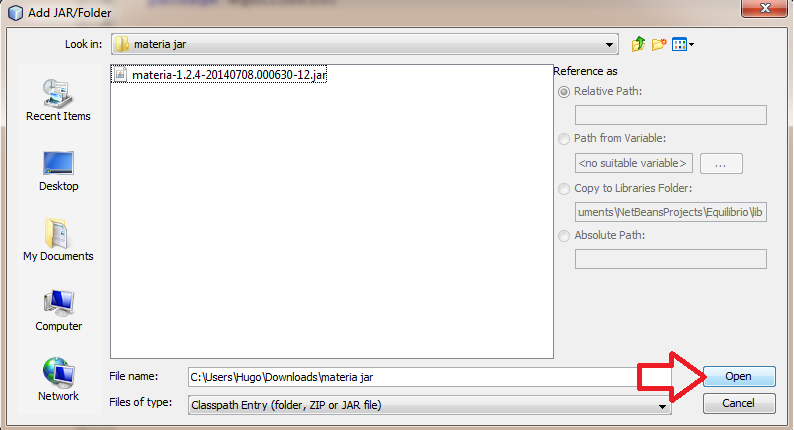
\includegraphics[scale=0.7]{select-materia-jar.png} 
			\end{center}

			Se puede ver entonces la librería agregada al proyecto.

			\begin{center}
			  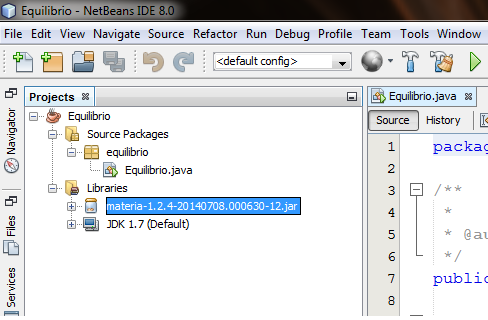
\includegraphics[scale=0.7]{library-added.png} 
			\end{center}
		\end{enumerate}

	\section{Maven}

		Desde maven utilizando el archivo pom.xml.
		    Crear nuevo proyecto :new proyect
		     Elegir la categoría ->Maven ->Java Applicationmaven java app
		    Elegir nombre del proyecto y dar click en finalizar.maven name
		    Podemos ver en la carpeta del proyecto la siguiente estructura
		\begin{verbatim}
		    Maven_Equilibrio
		    |-- pom.xml
		    `-- src
		        -- main
		           `-- java
		               `-- hugo
		                   `-- ejemplos
		                       `-- maven_equilibrio
		\end{verbatim}
		Abrimos el archivo pom.xml y agregamos las siguientes etiquetas


		\begin{lstlisting}[language=XML,morekeywords={repositories,
    repository,id,name,url,groupId,artifactId,dependencies,dependency}]
<dependencies>
  <dependency>
   <groupId>com.github.hugoredon</groupId>
   <artifactId>materia</artifactId>
   <version>1</version>
  </dependency>
</dependencies>
\end{lstlisting}


		5- Inmediatamente se ve agregada la dependencia Materia, cuando el proyecto se compile, se descargará el archivo jar automáticamente.

		maven materia added

		6.  Crear una clase java en cualquier paquete dentro de Source packages.maven create java class

		Escribimos dentro de esta clase el mismo código que en la entrada anterior.

	\section{Código}
		\begin{lstlisting}
			
		public class Equilibrio {
		 public static void main(String[] args) {
		 Compound agua = new Compound("agua");
		 agua.setCriticalTemperature(647.3);
		 agua.setCriticalPressure(2.212E7);
		 agua.setAcentricFactor(0.344861);
		 
		 Cubic cubicEquationOfState = EquationOfStateFactory.pengRobinsonBase();
		 Alpha alphaExpression = AlphaFactory.getStryjekAndVeraExpression();
		 
		 HeterogeneousSubstance substance =
		 new HeterogeneousSubstance(cubicEquationOfState, alphaExpression, agua);
		 double pressure = 101325;
		 substance.setPressure(pressure);
		 substance.bubbleTemperature();
		 double temperature = substance.getTemperature();
		 
		 System.out.println("(Presi|ó|n "+pressure+" [Pa])Temperatura de burbuja: " + temperature + "[K]");
		 }
		}

		\end{lstlisting}
		Ejecutamos el código y el resultado es:

		(Presión 101325.0 [Pa])Temperatura de burbuja: 374.5312063949659[K]
	\chapter{¿Cómo extender o modificar la librería desde el código fuente?}\label{chap:github}




\chapter{Solución de la ecuación de estado cúbica}\label{chap:cubicsolution}



\begin{equation}
z= \frac{P V}{R T}
\qquad
A=\frac{ap}{(RT)^2}
\qquad
B=\frac{bp}{RT}
\end{equation}

\begin{equation}
z^3-\left[1-(u-1)B\right]z^2+ \\ \left[A-uB-uB^2 +\\ wB^2\right]z-\left[AB+wB^2+wB^3\right]=0
\end{equation}


\begin{align}
\alpha &= 1-(u-1)B\\
\beta &= A -uB-uB^2+wB^3\\
\gamma &= AB +wB^2+ 2B^3\\
C &= 3\beta - \alpha^2\\
D&= - \alpha^3+ 4.5 \alpha \beta -13.5 \gamma\\
Q&=C^3+D^2
\end{align}


\begin{itemize}
\item Si $Q \leq 0 \qquad \vartheta = \arccos \left[\frac{-D}{\sqrt{-C^3}}\right]$
\begin{description}
\item{Líquido} $z = \frac{1}{3}\left[\alpha + 2 \sqrt{-C} \cos\left(\frac{\vartheta}{3} + 120\degree \right)\right]$
\item{Vapor} $z = \frac{1}{3}\left[\alpha + 2 \sqrt{-C} \cos\left(\frac{\vartheta}{3}\right)\right]$
\end{description}
Nota: En caso de que el z del líquido sea menor que B, entonces hay que calcularla como si fuera vapor.
\item Si $Q > 0 \qquad z = \frac{1}{3}\left[\alpha + \left(-D + \sqrt{Q}\right)^{\frac{1}{3}}+ \left(-D - \sqrt{Q}\right)^{\frac{1}{3}} \right]$
\end{itemize}
	\chapter{Ecuaciones}



\begin{equation}\label{eq:pressure}
P = \frac{R T}{v-b} - \frac{a}{v^2 +u b v + w b^2 }
\end{equation}


\begin{itemize}\itemsep0ex
\item $P$ : presión en $[Pa]$.
\item $v$ : volumen molar en $[\frac{m^3}{kg}]$
\item $a$ : Es una medida de la atracción entre las partículas. $[\frac{m^5}{kg s}]$
\item $b$ : volumen excluido por un mol de partículas.$[\frac{m^3}{kg}]$
\item $u$ y $w$ : Son los parámetros diferentes para cada ecuación de estado, ver tabla \ref{tab:cubics}
\item $R$ : Constante universal de los gases ideales en $\frac{m^3 Pa}{kgmol K}$
\end{itemize}


\begin{equation}\label{eq:a}
	b_i = \Omega_b \frac{R T_{ci}}{p_{ci}} 
\end{equation}

\begin{equation}\label{eq:b}
 a_i = \Omega_a \frac{\left(R T_{ci}\right)^2}{p_{ci}} \alpha_i
\end{equation}


\begin{equation}\label{eq:z}
z= \frac{P V}{R T}
\end{equation}

\begin{equation}\label{eq:volume}
V = \frac{R T}{z P}
\end{equation}

\begin{equation}\label{eq:AB}
A=\frac{ap}{(RT)^2}
\qquad
B=\frac{bp}{RT}
\end{equation}

\begin{equation}
z^3-\left[1-(u-1)B\right]z^2+ \\ \left[A-uB-uB^2 +\\ wB^2\right]z-\left[AB+wB^2+wB^3\right]=0
\end{equation}


\subsubsection{Entalpía del gas ideal}
\begin{equation}\label{eq:idealgasenthalpy}
h^{\neq} = \sum_{i=1}^{nc} x_i \left[ h_i^{ref} + \int_{Tref}^{T} Cp_i^{\neq} \mathrm{d}T \right]
\end{equation}

\section{Entalpía}
\begin{equation}\label{eq:enthalpy}
h = h^{\neq} + \left[ \frac{T(\frac{\partial a}{\partial T}) - a}{b\sqrt{u²-4w} }\right] 
\ln\left[\frac{2v+b\left(u + \sqrt{u²-4w}\right)}{2v+b\left(u - \sqrt{u²-4w}\right)}\right]
+ pv - RT
\end{equation}

\begin{lstlisting}[label=some-code,caption=Some Code]
private  double calculateEnthalpy( double volume){
    double idealGasEnthalpy = calculateIdealGasEnthalpy();
    double a = calculate_a_cubicParameter();
    double b = calculate_b_cubicParameter();
    double L = cubicEquationOfState.calculateL(volume, b);
    double partial_aPartial_temperature = partial_aPartial_temperature( );
    
    return idealGasEnthalpy + ((partial_aPartial_temperature - a)/b) * L  + pressure * volume - Constants.R *temperature;
}
\end{lstlisting}	



\subsection{Entropía}
\begin{equation}
s = s^{\neq} + R\ln\left[\frac{z(v-b)}{v}\right] + \frac{\frac{\partial a}{\partial T}}{b \sqrt{u^2 - 4w}}
\ln\left[\frac{2v+b\left(u + \sqrt{u²-4w}\right)}{2v+b\left(u - \sqrt{u²-4w}\right)}\right]
\end{equation}
\begin{equation}
s^{\neq} = \sum_{i=1}^{nc} x_i\left[s_i^{ref} + \int_{Tref}^T \frac{Cp_i^{\neq}}{T} \mathrm{d}T 
- R\ln \left(\frac{p}{p_{ref}}\right)- R\ln{x_i}
\right]
\end{equation}


\begin{equation}\label{eq:gibbs}
g = h - T * s;
\end{equation}


\begin{multline}\label{eq:fugacity}
\ln\hat{\phi_i} = - \ln\left(\frac{v-b}{v}\right) 
+ (z-1)\left[\frac{1}{b}\frac{\partial bN}{\partial N_i}\right]
+ \frac{a}{RTb\sqrt{u^2-4w}}
\\
\left[\frac{1}{b}\frac{\partial bN}{\partial N_i}
- \frac{1}{aN}\frac{\partial aN²}{\partial N_i}\right]
\ln\left[\frac{2v+b\left(u + \sqrt{u²-4w}\right)}{2v+b\left(u - \sqrt{u²-4w}\right)}\right]
-\ln{z}
\end{multline}
	\chapter{Herramientas para la página de internet}\label{chap:webTools}

\begin{itemize}
	\item Java Enterprise Edition
	\item Java Server Faces
	\item Hibernate
	\item MySQL
	\item Enterprise Java Beans 3
	\item Wildfly
	\item Openshift
	\item HTML, CSS
	\item Javascript JQuery
\end{itemize}


\section{Openshift}
		OpenShift es una plataforma de programación en la nube orientada a servicios de Red Hat. Una versión para la nube privada se llama OpenShift Enterprise. El software que ejecuta el servicio se encuentra bajo el nombre `OpenShift Origin' de código abierto y está disponible en GitHub.

\section{Wildfly}
	WildFly, anteriormente conocido como `JavaBeans Open Source Software Application Server' es un servidor de aplicaciones que implementa la plataforma Java Enterprise Edition. JBoss está escrito en Java y como tal es multiplataforma: utilizable en cualquier sistema operativo que soporte Java
	\subsection{Expresiones de $\alpha$}

	\subsubsection{Soave\cite{soave}}

\begin{gather}
	\alpha^{\nicefrac{1}{2}} = 1 + m \left(1-\sqrt{T_r}\right)\\
	m = 0.48508+1.55171\omega-0.15613\omega^2
\end{gather}
	\subsubsection{Peng and Robinson \cite{pengRobinson}}


\begin{gather}
	\alpha^{\nicefrac{1}{2}} = 1 + m \left(1-\sqrt{T_r}\right)\\
	m = 0.37464+1.54226\omega-0.2699\omega^2
\end{gather}
	\subsubsection{Mathias\cite{mathias} }
\begin{itemize}

\item{$T < T_C$}
\begin{gather}
	\alpha^{\nicefrac{1}{2}} = 1 + m \left(1-\sqrt{T_r}\right)- A\left(1-T_r\right)\left(0.7-T_r\right)
	\\
	m = 0.48508+1.55191\omega-0.15613\omega^2
\end{gather}

\item{$T > T_c$}
\begin{gather}
	\alpha = \exp{\left[ \left( \frac{c-1}{c} \right)  \left(  1- T_r^c  \right)  \right]}\\
	c = 1 + \frac{m}{2} + 0.3 A
\end{gather}

 \end{itemize}


	\subsubsection{Stryjek and Vera(PRSV)\cite{stryjekVeraPureCompounds} }
\begin{itemize}

\item{$T < T_C$}
\begin{gather}
	\alpha^{\nicefrac{1}{2}} = 1 + \kappa_0 \left(1-\sqrt{T_r}\right)- \kappa_1\left(1-T_r\right)\left(0.7-T_r\right)
	\\
	\kappa_0 = 0.378893+1.4897153\omega-0.17131848\omega^2+0.0196554\omega³
\end{gather}

\item{$T > T_c$}
\begin{equation}
	\alpha^{\nicefrac{1}{2}} = 1 + \kappa_0\left(1- \sqrt{T_r}\right)
\end{equation}

 \end{itemize}	
	\subsubsection{Adachi and Lu \cite{adachiLu}}

\begin{equation}
\alpha = A\cdot {10}^{B\left(1-T_r\right)}
\end{equation}
	\subsubsection{Soave \cite{soaveR}}

\begin{equation}\label{eq:soaveR}
\alpha= 1+\left(1-T_r\right)\left(A + \frac{B}{T_r}\right)
\end{equation}
	\subsubsection{Melhem, et al.\cite{melhem}}

\begin{equation}
\ln{\alpha}=A\left(1-T_r\right)+ B\left(1-\sqrt{T_r}\right)^2
\end{equation}
	\subsubsection{Androulakis,et al.\cite{androulakis}}

\begin{itemize}
\item{$T < T_C$}
\begin{equation}
 \alpha = 1 + A \left(1-T_r^{\nicefrac{2}{3}}\right) + B\left(1-T_r^{\nicefrac{2}{3}}\right)^2+ C\left(1-T_r^{\nicefrac{2}{3}}\right)^3
\end{equation}
\item{$T > T_c$}
\begin{equation}
\alpha = \mathrm{e}^{A\left(1-T_r^{\nicefrac{2}{3}}\right)}
\end{equation}
\end{itemize}
	\subsubsection{Mathias and Copeman. \cite{mathiasCopeman,michelsen}}

\begin{itemize}
\item{$T < T_c$}
\begin{equation}
\alpha^{\nicefrac{1}{2}} = 1 + A\left(1-\sqrt{T_r}\right) + B\left(1-\sqrt{T_r}\right)^2 + C\left(1-\sqrt{T_r}\right)^3
\end{equation}
\item{$T > T_c$}
\begin{equation}
\alpha^{\nicefrac{1}{2}} = 1 + A\left(1-\sqrt{T_r}\right)
\end{equation}
\footnote{La ecuación no se incluyó en el trabajo original de Mathias and Copeman\cite{mathiasCopeman}; esta expresión fue incorporada en el trabajo de Dahl and Michelsen \cite{michelsen}}
\end{itemize}
	\subsubsection{Yu and Lu\cite{yuLu}}

\begin{itemize}
\item{$T < T_c$}
\begin{equation}
 \log_{10}{\alpha} = \left(A+B T_r+ C T_r^2\right)\left(1-T_r\right)
\end{equation}
\item{$T > T_c$}
\begin{equation}
 \log_{10}{\alpha} = \left(A+B+C \right)\left(1-T_r\right)
\end{equation}
\end{itemize}
	\subsubsection{Stryjek and Vera\cite{stryjekVera}}

\begin{itemize}
\item{$T < T_c$}
\begin{gather}
\alpha^{\nicefrac{1}{2}} = 1 + \kappa\left(1-\sqrt{T_r}\right)\\
\kappa = m + \left[
		A+ B\left(C- T_r\right)\left(1-\sqrt{T_r}\right)
	\right]
	\left[
		\left(1+ \sqrt{T_r}\right)\left(0.7-T_r\right)
	\right]\\
m=0.378893 + 1.4897153 \omega - 0.17131848 \omega^2+ 0.0196554 \omega^3
\end{gather}
\item{$T > T_c$}
\begin{equation}
\alpha^{\nicefrac{1}{2}} = 1 + m\left(1-\sqrt{T_r}\right)
\end{equation}
\end{itemize}
	\subsubsection{Twu\cite{twuequation}}
\begin{equation}
	\alpha = T_r^{N\left(M-1\right)}\exp{\left(L\left(1-T_r^{N M}\right)\right)}
\end{equation}
	\subsubsection{Twu \cite{twuactivity}}
\begin{itemize}
\item{$T < T_c$}
\begin{gather}
\alpha = \alpha^{(0)} + \omega\left(\alpha^{(1)}-\alpha^{(0)}\right)\\
\text{Para}\qquad \alpha^{(0)}\notag\\
L= 0.196545\qquad M=0.906437\qquad N=1.26251\\
\text{Para}\qquad \alpha^{(1)}\notag\\
L=0.704001 \qquad M =0.790407 \qquad N=2.13076
\end{gather}
\item{$T > T_c$}
\begin{gather}
\alpha = \alpha^{(0)} + \omega\left(\alpha^{(1)}-\alpha^{(0)}\right)\\
\text{Para}\qquad \alpha^{(0)}\notag\\
L= 0.358826\qquad M=4.23478\qquad N=-0.2\\
\text{Para}\qquad \alpha^{(1)}\notag\\
L=0.0206444 \qquad M =1.22942 \qquad N=-8.0
\end{gather}
\end{itemize}
	\subsubsection{GCEOS (AspenHYSYS)}

\begin{gather}
\alpha^{\nicefrac{1}{2}} = 1 + \kappa \left(1 - \sqrt{T_r}\right)\\
\kappa = \kappa_0 + \left[ 
	\kappa_1 + \left(   \kappa_2 - \kappa_3 T_r   \right)
	\left(1 - T_r^{\kappa_4}\right) 
\right]
\left[
	\left(1 + \sqrt{T_r}\right)\left(0.7 - T_r\right)
\right]
T^{\kappa_5}\\
\kappa_0 = A + B \omega+ C \omega^2+ D \omega^3
\end{gather}





	\bibliographystyle{babplain}
	\bibliography{bib/bibliography}  
\end{document} 